\documentclass[]{book}
\usepackage{lmodern}
\usepackage{amssymb,amsmath}
\usepackage{ifxetex,ifluatex}
\usepackage{fixltx2e} % provides \textsubscript
\ifnum 0\ifxetex 1\fi\ifluatex 1\fi=0 % if pdftex
  \usepackage[T1]{fontenc}
  \usepackage[utf8]{inputenc}
\else % if luatex or xelatex
  \ifxetex
    \usepackage{mathspec}
  \else
    \usepackage{fontspec}
  \fi
  \defaultfontfeatures{Ligatures=TeX,Scale=MatchLowercase}
\fi
% use upquote if available, for straight quotes in verbatim environments
\IfFileExists{upquote.sty}{\usepackage{upquote}}{}
% use microtype if available
\IfFileExists{microtype.sty}{%
\usepackage{microtype}
\UseMicrotypeSet[protrusion]{basicmath} % disable protrusion for tt fonts
}{}
\usepackage[margin=1in]{geometry}
\usepackage{hyperref}
\hypersetup{unicode=true,
            pdftitle={GEO880: Patterns and Trends in Environmental Data},
            pdfauthor={Patrick Laube and Nils Ratnaweera},
            pdfborder={0 0 0},
            breaklinks=true}
\urlstyle{same}  % don't use monospace font for urls
\usepackage{color}
\usepackage{fancyvrb}
\newcommand{\VerbBar}{|}
\newcommand{\VERB}{\Verb[commandchars=\\\{\}]}
\DefineVerbatimEnvironment{Highlighting}{Verbatim}{commandchars=\\\{\}}
% Add ',fontsize=\small' for more characters per line
\usepackage{framed}
\definecolor{shadecolor}{RGB}{248,248,248}
\newenvironment{Shaded}{\begin{snugshade}}{\end{snugshade}}
\newcommand{\KeywordTok}[1]{\textcolor[rgb]{0.13,0.29,0.53}{\textbf{{#1}}}}
\newcommand{\DataTypeTok}[1]{\textcolor[rgb]{0.13,0.29,0.53}{{#1}}}
\newcommand{\DecValTok}[1]{\textcolor[rgb]{0.00,0.00,0.81}{{#1}}}
\newcommand{\BaseNTok}[1]{\textcolor[rgb]{0.00,0.00,0.81}{{#1}}}
\newcommand{\FloatTok}[1]{\textcolor[rgb]{0.00,0.00,0.81}{{#1}}}
\newcommand{\ConstantTok}[1]{\textcolor[rgb]{0.00,0.00,0.00}{{#1}}}
\newcommand{\CharTok}[1]{\textcolor[rgb]{0.31,0.60,0.02}{{#1}}}
\newcommand{\SpecialCharTok}[1]{\textcolor[rgb]{0.00,0.00,0.00}{{#1}}}
\newcommand{\StringTok}[1]{\textcolor[rgb]{0.31,0.60,0.02}{{#1}}}
\newcommand{\VerbatimStringTok}[1]{\textcolor[rgb]{0.31,0.60,0.02}{{#1}}}
\newcommand{\SpecialStringTok}[1]{\textcolor[rgb]{0.31,0.60,0.02}{{#1}}}
\newcommand{\ImportTok}[1]{{#1}}
\newcommand{\CommentTok}[1]{\textcolor[rgb]{0.56,0.35,0.01}{\textit{{#1}}}}
\newcommand{\DocumentationTok}[1]{\textcolor[rgb]{0.56,0.35,0.01}{\textbf{\textit{{#1}}}}}
\newcommand{\AnnotationTok}[1]{\textcolor[rgb]{0.56,0.35,0.01}{\textbf{\textit{{#1}}}}}
\newcommand{\CommentVarTok}[1]{\textcolor[rgb]{0.56,0.35,0.01}{\textbf{\textit{{#1}}}}}
\newcommand{\OtherTok}[1]{\textcolor[rgb]{0.56,0.35,0.01}{{#1}}}
\newcommand{\FunctionTok}[1]{\textcolor[rgb]{0.00,0.00,0.00}{{#1}}}
\newcommand{\VariableTok}[1]{\textcolor[rgb]{0.00,0.00,0.00}{{#1}}}
\newcommand{\ControlFlowTok}[1]{\textcolor[rgb]{0.13,0.29,0.53}{\textbf{{#1}}}}
\newcommand{\OperatorTok}[1]{\textcolor[rgb]{0.81,0.36,0.00}{\textbf{{#1}}}}
\newcommand{\BuiltInTok}[1]{{#1}}
\newcommand{\ExtensionTok}[1]{{#1}}
\newcommand{\PreprocessorTok}[1]{\textcolor[rgb]{0.56,0.35,0.01}{\textit{{#1}}}}
\newcommand{\AttributeTok}[1]{\textcolor[rgb]{0.77,0.63,0.00}{{#1}}}
\newcommand{\RegionMarkerTok}[1]{{#1}}
\newcommand{\InformationTok}[1]{\textcolor[rgb]{0.56,0.35,0.01}{\textbf{\textit{{#1}}}}}
\newcommand{\WarningTok}[1]{\textcolor[rgb]{0.56,0.35,0.01}{\textbf{\textit{{#1}}}}}
\newcommand{\AlertTok}[1]{\textcolor[rgb]{0.94,0.16,0.16}{{#1}}}
\newcommand{\ErrorTok}[1]{\textcolor[rgb]{0.64,0.00,0.00}{\textbf{{#1}}}}
\newcommand{\NormalTok}[1]{{#1}}
\usepackage{longtable,booktabs}
\usepackage{graphicx,grffile}
\makeatletter
\def\maxwidth{\ifdim\Gin@nat@width>\linewidth\linewidth\else\Gin@nat@width\fi}
\def\maxheight{\ifdim\Gin@nat@height>\textheight\textheight\else\Gin@nat@height\fi}
\makeatother
% Scale images if necessary, so that they will not overflow the page
% margins by default, and it is still possible to overwrite the defaults
% using explicit options in \includegraphics[width, height, ...]{}
\setkeys{Gin}{width=\maxwidth,height=\maxheight,keepaspectratio}
\IfFileExists{parskip.sty}{%
\usepackage{parskip}
}{% else
\setlength{\parindent}{0pt}
\setlength{\parskip}{6pt plus 2pt minus 1pt}
}
\setlength{\emergencystretch}{3em}  % prevent overfull lines
\providecommand{\tightlist}{%
  \setlength{\itemsep}{0pt}\setlength{\parskip}{0pt}}
\setcounter{secnumdepth}{5}
% Redefines (sub)paragraphs to behave more like sections
\ifx\paragraph\undefined\else
\let\oldparagraph\paragraph
\renewcommand{\paragraph}[1]{\oldparagraph{#1}\mbox{}}
\fi
\ifx\subparagraph\undefined\else
\let\oldsubparagraph\subparagraph
\renewcommand{\subparagraph}[1]{\oldsubparagraph{#1}\mbox{}}
\fi

%%% Use protect on footnotes to avoid problems with footnotes in titles
\let\rmarkdownfootnote\footnote%
\def\footnote{\protect\rmarkdownfootnote}

%%% Change title format to be more compact
\usepackage{titling}

% Create subtitle command for use in maketitle
\newcommand{\subtitle}[1]{
  \posttitle{
    \begin{center}\large#1\end{center}
    }
}

\setlength{\droptitle}{-2em}
  \title{GEO880: Patterns and Trends in Environmental Data}
  \pretitle{\vspace{\droptitle}\centering\huge}
  \posttitle{\par}
  \author{Patrick Laube and Nils Ratnaweera}
  \preauthor{\centering\large\emph}
  \postauthor{\par}
  \date{}
  \predate{}\postdate{}


\usepackage{amsthm}
\newtheorem{theorem}{Theorem}[chapter]
\newtheorem{lemma}{Lemma}[chapter]
\theoremstyle{definition}
\newtheorem{definition}{Definition}[chapter]
\newtheorem{corollary}{Corollary}[chapter]
\newtheorem{proposition}{Proposition}[chapter]
\theoremstyle{definition}
\newtheorem{example}{Example}[chapter]
\theoremstyle{definition}
\newtheorem{exercise}{Exercise}[chapter]
\theoremstyle{remark}
\newtheorem*{remark}{Remark}
\newtheorem*{solution}{Solution}
\begin{document}
\maketitle

{
\setcounter{tocdepth}{1}
\tableofcontents
}
\chapter*{Introduction Chapter}\label{introduction-chapter}
\addcontentsline{toc}{chapter}{Introduction Chapter}

For our practical \texttt{R} course building-up skills for analyzing
movement data in the software environment \texttt{R}, you'll be using
data from the ZHAW project
\href{https://www.zhaw.ch/de/lsfm/institute-zentren/iunr/integrative-oekologie/wildtiermanagement/referenzprojekte/}{``Prävention
von Wildschweinschäden in der Landwirtschaft''}.

The project investigates the spatiotemporal movement patterns of wild
boar (\emph{Sus scrofa}) in agricultural landscapes. For more
information you can ask
\href{https://www.zhaw.ch/de/ueber-uns/person/sigb/}{Beni Sigrist}, one
of the course participants involved in this project. We will study the
trajectories of these wild boar, practicing the most basic analysis
tasks of Computational Movement Analysis (CMA).

\textbf{Please note} we are given application data from an ongoing
research project. Capturing wild living animals and then equipping them
with GPS collars is a very labor and cost intensive form of research.
Consequently, data resulting such campaigns is a very valuable asset
that must be protected. So, please do not pass on this data, for any use
beyond this module contact Patrick Laube or the data owner Stefan Suter
(\href{mailto:suts@zhaw.ch}{\nolinkurl{suts@zhaw.ch}}).

\chapter{Exercise 1}\label{exercise-1}

Exercise 1 covers the necessary steps for getting ready in \texttt{R}
and some basic concepts for setting up a well-structured \texttt{R}
project. The lesson introduces how additional packages that provide
useful functions for data science are made available and how spatial
data is handled. The exercise concludes with the creation of your first
map featuring movement data.

\section{Leaning outcomes}\label{leaning-outcomes}

\begin{itemize}
\tightlist
\item
  You learn how to structure an \texttt{R} project.
\item
  You can read movement data from a .csv-file into a \texttt{data.frame}
\item
  You can convert spatial point data from a \texttt{data.frame} to a
  spatial object \texttt{sf}
\item
  You can perform basic spatial operations on spatial objects in
  \texttt{R}
\item
  You can produce simple maps of your spatial data using
  \texttt{ggplot2}
\end{itemize}

\section{Prerequisites}\label{prerequisites}

Readings Skills from ``R for Data Science'' (Wickham and Grolemund
2017):

\begin{itemize}
\tightlist
\item
  RS1.1 Preface (16p, ix-xxiv)
\item
  RS1.2 Chap2 Workflow basics (3p, 37-39)
\item
  RS1.3 Chap4 Workflow scripts (3p, 77-79)
\item
  RS1.4 Chap6 workflow projects (6p, 111-116)
\item
  RS1.5 Chap8 Data Import with \texttt{readr} (21p)
\item
  RS1.6 Chap13 Date and Times with \texttt{lubridate} (18p, 237-256)
\end{itemize}

\section{Preperation}\label{preperation}

If you haven't already, install the packages \texttt{tidyverse}, and
\texttt{devtools} (using \texttt{install.packages()}). Use
\texttt{devtools} to install the newest version of
\texttt{ggplot}\footnote{We will need the newest version of
  \texttt{ggplot2} to plot spatial \texttt{sf} objects.} from github
(see code below). Additionally, install the packages
\texttt{sf}\footnote{If you are working on RStudio Server, you will need
  to install \texttt{udunits2} with some additional parameters (see code
  example).}, \texttt{raster} and \texttt{ggspatial}. \textbf{Restart
your \texttt{R} session after installing all these packages.}

\begin{Shaded}
\begin{Highlighting}[]
\KeywordTok{install.packages}\NormalTok{(}\StringTok{"tidyverse"}\NormalTok{)}
\KeywordTok{install.packages}\NormalTok{(}\StringTok{"devtools"}\NormalTok{)}
\NormalTok{devtools::}\KeywordTok{install_github}\NormalTok{(}\StringTok{"tidyverse/ggplot2"}\NormalTok{)}

\CommentTok{# run the following line only if you are working on RStudio Server}
\KeywordTok{install.packages}\NormalTok{(}\StringTok{'udunits2'}\NormalTok{, }\DataTypeTok{type =} \StringTok{"source"}\NormalTok{, }\DataTypeTok{repo =} \StringTok{"cran.rstudio.com"}\NormalTok{, }\DataTypeTok{configure.args=}\StringTok{"--with-udunits2-include=/usr/include/udunits2"}\NormalTok{)}

\KeywordTok{install.packages}\NormalTok{(}\StringTok{"sf"}\NormalTok{)}



\KeywordTok{install.packages}\NormalTok{(}\StringTok{"raster"}\NormalTok{)}
\KeywordTok{install.packages}\NormalTok{(}\StringTok{"ggspatial"}\NormalTok{)}
\end{Highlighting}
\end{Shaded}

\section{Tasks and inputs}\label{tasks-and-inputs}

\subsection{Task 1: Initialize project}\label{task-1-initialize-project}

Create a new \emph{RStudio Project}. As recommended in Wickham and
Grolemund (2017), remove the option ``\emph{Restore .RData into
workspace at startup}'' and set the option ``\emph{save workspace to
.RData on exit}'' to ``\emph{Never}''.

Create a new R-File and divide it into the sections necessary in a
classical Data Science Workflow. We recommend following sections:

\begin{itemize}
\tightlist
\item
  Loading environment / libraries
\item
  Data import
\item
  Data cleansing
\item
  Data analysis and visualization
\end{itemize}

``Sections'' can be created within RStudio by adding Comments
(\texttt{\#}) with at least 4 trailing dashes (\texttt{-}), equal signs
(\texttt{=}), or pound signs (\texttt{\#}). Sections allow code folding
(try clicking on the small triangle next to the line number) and
facilitate navigation (try the shortcut:
\texttt{Shift}+\texttt{Alt}+\texttt{J}).

Load the package \texttt{tidyverse} in the appropriate section.

\subsection{Task 2: Import data}\label{task-2-import-data}

In section ``data import'', import the file
\texttt{wildschwein\_BE.csv}.

Note:

\begin{itemize}
\tightlist
\item
  If your are using
  \href{https://support.rstudio.com/hc/en-us/articles/218611977-Importing-Data-with-RStudio}{a
  graphical tool} to import your code, make sure you save the
  corresponding code in your R Script. This is important in regard to
  the reproducibility of your script and will ensure that your workflow
  is documented without gaps. We'd rather recommend to move away from
  using graphical tools and focus on using code.
\item
  We recommend using one of the \texttt{tidyverse} functions
  (\texttt{read\_*}) to import your data. These functions are less error
  prone than the base \texttt{R} functions (\texttt{read.*}).
  Specifically for the wild boar data, we recommend
  \texttt{read\_delim()}.
\item
  If you use \texttt{read\_delim()} and receive warnings during import,
  have a look at these warnings by using the function
  \texttt{problems()}. Resolve these problems until import runs without
  warnings.
\item
  Assign correct data types as necessary and make sure the time zone is
  set correctly for the date/time column.
\item
  For everyone working on the RStudio Server: You will first need to
  upload this data to the server using the ``\emph{upload}''-button in
  the ``\emph{Files}'' tab.
\end{itemize}

\subsection{Task 3: Explore Data}\label{task-3-explore-data}

We will use a range of different plotting techniques in this course.
Several plotting techniques have emerged in recent years, each with
their specific strengths and weaknesses. While \texttt{base::plot()}is
quick and simple, it not very scalable with growing complexity.
\texttt{ggplot} offers solutions for most use cases and has a elegant
syntax that is easy to get accustomed to. We will get to know other
techniques later in the course.

Get an overview of your data by creating a first ``map-like'' plot of
your data producing a simple scatter plot with \texttt{ggplot}. Do you
spot outliers? If so, get rid of the outliers and plot your data again
without outliers.

Setting up a \texttt{ggplot} with our data is done using the command
\texttt{ggplot(wildschwein\_BE,\ aes(Long,\ Lat,\ colour\ =\ TierID))}.
Creating a map is done via the basic scatter plot command
\texttt{geom\_point()}. Use \texttt{coord\_map()} to get a reasonable
aspect ratio of \texttt{Lat} and \texttt{Long}. Assigning every
individual its own colour is done using the \texttt{ggplot} argument
\texttt{colour\ =}.

Save your code in the appropriate section.

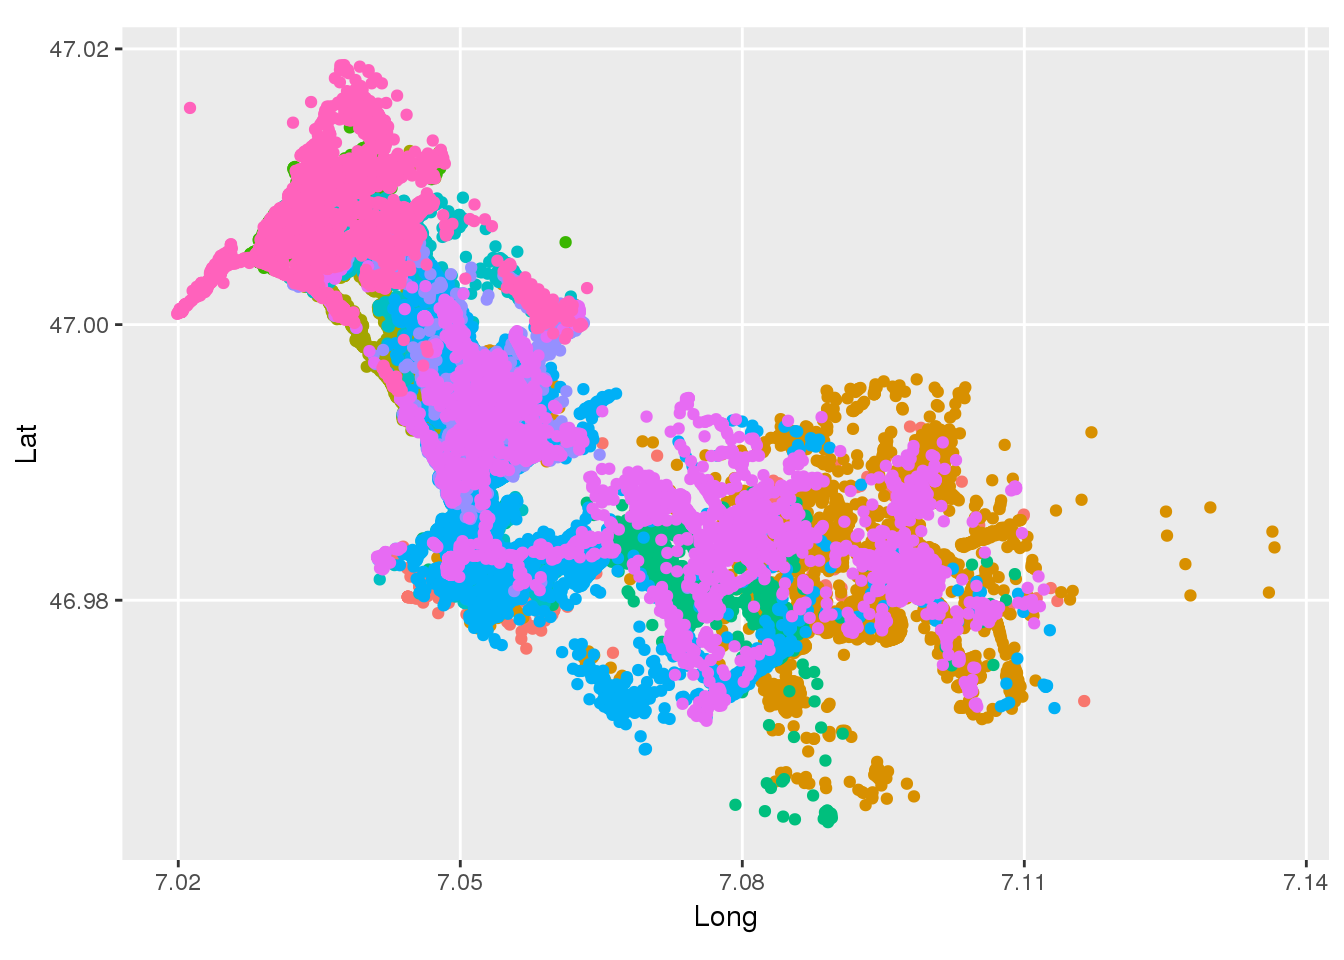
\includegraphics{_main_files/figure-latex/unnamed-chunk-5-1.pdf}

\subsection{Input: Handling spatial
data}\label{input-handling-spatial-data}

Until now, we've handled spatial data within data frames. This works
well for many tasks, but sometimes we need special \emph{spatial}
classes to handle our trajectories. We will get to now such cases in our
next tasks, but first we need to convert our \texttt{data.frame} into a
spatial object. Some of you might be familiar with the \texttt{sp}
package with the classes \texttt{SpatialPoints},
\texttt{SpatialPointsDataFrame} and so on. Just recently the new and
exiting package \texttt{sf}, was released on CRAN. \texttt{sf} has some
huge advantages over sp:

\begin{itemize}
\tightlist
\item
  simple features are essentially data frames, which mean they interface
  with the \texttt{tidyverse}\\
\item
  comply with the common Open Geospatial Consortium (OGC) standards (ISO
  19125-1:2004) and interface with other important spatial tools such as
  GDAL, PostGIS, GeoJSON and so fourth
\item
  are being rapidly implemented in visualisation tools such as
  \texttt{ggplot2}, \texttt{plotly} and \texttt{tmap}
\end{itemize}

We will largely rely on \texttt{sf}when working with vector data in
\texttt{R}. In order to transform our \texttt{data.frame} into an sf
object, we need to use the function \texttt{st\_as\_sf()} while
specifying the columns storing the coordinates and the coordinate
reference system\footnote{At this point, we assume you know what a
  Coordinate Reference Systems is. Check out
  \href{https://earthdatascience.org/courses/earth-analytics/spatial-data-r/intro-to-coordinate-reference-systems/}{this
  link} if this is not the case.}.

\begin{Shaded}
\begin{Highlighting}[]

\KeywordTok{library}\NormalTok{(sf)}

\NormalTok{wildschwein_BE_sf <-}\StringTok{ }\KeywordTok{st_as_sf}\NormalTok{(wildschwein_BE, }\DataTypeTok{coords =} \KeywordTok{c}\NormalTok{(}\StringTok{"Long"}\NormalTok{, }\StringTok{"Lat"}\NormalTok{), }\DataTypeTok{crs =} \DecValTok{4326}\NormalTok{)}
\end{Highlighting}
\end{Shaded}

Notice how \texttt{st\_as\_sf} takes the EPSG code for the
\texttt{crs\ =} argument. This is so much easier and more elegant than
using \texttt{PROJ.4} or \texttt{WKT}. You can find a lot of useful
information on Coordinate Reference Systems (including EPSG Codes ,
etc.) under
\href{http://spatialreference.org/ref/epsg/2056/}{spatialreference.org}
or \url{http://epsg.io}.

Let's compare our original \texttt{data.frame} with this new \texttt{sf}
object:

\begin{Shaded}
\begin{Highlighting}[]
\NormalTok{wildschwein_BE}
\end{Highlighting}
\end{Shaded}

\begin{verbatim}
## # A tibble: 141,763 x 6
##    TierID TierName CollarID DatetimeUTC           Lat  Long
##    <chr>  <chr>       <int> <dttm>              <dbl> <dbl>
##  1 001A   Ueli        12272 2014-05-28 21:01:14  47.0  7.05
##  2 001A   Ueli        12272 2014-05-28 21:15:18  47.0  7.05
##  3 001A   Ueli        12272 2014-05-28 21:30:13  47.0  7.05
##  4 001A   Ueli        12272 2014-05-28 21:45:11  47.0  7.05
##  5 001A   Ueli        12272 2014-05-28 22:00:33  47.0  7.05
##  6 001A   Ueli        12272 2014-05-28 22:15:16  47.0  7.05
##  7 001A   Ueli        12272 2014-05-28 22:30:14  47.0  7.05
##  8 001A   Ueli        12272 2014-05-28 22:45:09  47.0  7.05
##  9 001A   Ueli        12272 2014-05-28 23:00:12  47.0  7.05
## 10 001A   Ueli        12272 2014-05-28 23:15:08  47.0  7.05
## # ... with 141,753 more rows
\end{verbatim}

\begin{Shaded}
\begin{Highlighting}[]
\NormalTok{wildschwein_BE_sf}
\end{Highlighting}
\end{Shaded}

\begin{verbatim}
## Simple feature collection with 141763 features and 4 fields
## geometry type:  POINT
## dimension:      XY
## bbox:           xmin: 7.019889 ymin: 46.96389 xmax: 7.136615 ymax: 47.01882
## epsg (SRID):    4326
## proj4string:    +proj=longlat +datum=WGS84 +no_defs
## # A tibble: 141,763 x 5
##    TierID TierName CollarID DatetimeUTC                    geometry
##    <chr>  <chr>       <int> <dttm>                      <POINT [°]>
##  1 001A   Ueli        12272 2014-05-28 21:01:14 (7.049359 46.99378)
##  2 001A   Ueli        12272 2014-05-28 21:15:18 (7.049342 46.99383)
##  3 001A   Ueli        12272 2014-05-28 21:30:13 (7.049367 46.99379)
##  4 001A   Ueli        12272 2014-05-28 21:45:11 (7.049329 46.99383)
##  5 001A   Ueli        12272 2014-05-28 22:00:33 (7.049336 46.99376)
##  6 001A   Ueli        12272 2014-05-28 22:15:16 (7.049282 46.99385)
##  7 001A   Ueli        12272 2014-05-28 22:30:14 (7.049401 46.99381)
##  8 001A   Ueli        12272 2014-05-28 22:45:09  (7.051912 46.9958)
##  9 001A   Ueli        12272 2014-05-28 23:00:12  (7.051797 46.9958)
## 10 001A   Ueli        12272 2014-05-28 23:15:08 (7.051658 46.99582)
## # ... with 141,753 more rows
\end{verbatim}

As you can see, \texttt{st\_as\_sf()} has added some metadata to our
dataframe (\texttt{geometry\ type}, \texttt{dimension}, \texttt{bbox},
\texttt{epsg} and \texttt{proj4string}) and replaced the columns
\texttt{Lat} and \texttt{Long} with a column named \texttt{geometry}.
Other than that, the new \texttt{sf} object is very similar to our
original dataframe. In fact, \texttt{sf} objects \emph{are} essentially
\texttt{dataframes}, just ask \texttt{R}:

\begin{Shaded}
\begin{Highlighting}[]
\KeywordTok{is.data.frame}\NormalTok{(wildschwein_BE_sf)}
\NormalTok{## [1] TRUE}
\end{Highlighting}
\end{Shaded}

All operations we know from handling \texttt{data.frames} can be used on
the \texttt{sf} object. Try some out!

\begin{Shaded}
\begin{Highlighting}[]
\CommentTok{# subset rows}
\NormalTok{wildschwein_BE_sf[}\DecValTok{1}\NormalTok{:}\DecValTok{10}\NormalTok{,]}
\NormalTok{wildschwein_BE_sf[wildschwein_BE_sf$TierName ==}\StringTok{ "Ueli"}\NormalTok{,]}

\CommentTok{# subset colums}
\NormalTok{wildschwein_BE_sf[,}\DecValTok{2}\NormalTok{:}\DecValTok{3}\NormalTok{]}
\end{Highlighting}
\end{Shaded}

Instead of keeping the same data twice (once as a \texttt{data.frame},
and once as an \texttt{sf} object), we will overwrite the
\texttt{data.frame} and continue working with the \texttt{sf} object
from now on. This saves some memory space in \texttt{R} and avoids
confusion. It is however, unideal that the \texttt{st\_as\_sf()}
operation \emph{replaced} the \texttt{Lat} and \texttt{Long} columns
with the \texttt{geometry} column. It would be helpful to retain the
\texttt{Lat}/\texttt{Long} columns and have the \texttt{geometry} column
\emph{in addition}. We can enforce this by using the argument
\texttt{remove\ =\ FALSE}.

\begin{Shaded}
\begin{Highlighting}[]
\NormalTok{wildschwein_BE =}\StringTok{ }\KeywordTok{st_as_sf}\NormalTok{(wildschwein_BE, }\DataTypeTok{coords =} \KeywordTok{c}\NormalTok{(}\StringTok{"Long"}\NormalTok{, }\StringTok{"Lat"}\NormalTok{), }\DataTypeTok{crs =} \DecValTok{4326}\NormalTok{,}\DataTypeTok{remove =} \OtherTok{FALSE}\NormalTok{)}

\NormalTok{wildschwein_BE }\CommentTok{# note how the Lat/Long information is stored twice}
\NormalTok{## Simple feature collection with 141763 features and 6 fields}
\NormalTok{## geometry type:  POINT}
\NormalTok{## dimension:      XY}
\NormalTok{## bbox:           xmin: 7.019889 ymin: 46.96389 xmax: 7.136615 ymax: 47.01882}
\NormalTok{## epsg (SRID):    4326}
\NormalTok{## proj4string:    +proj=longlat +datum=WGS84 +no_defs}
\NormalTok{## # A tibble: 141,763 x 7}
\NormalTok{##    TierID TierName CollarID DatetimeUTC           Lat  Long}
\NormalTok{##    <chr>  <chr>       <int> <dttm>              <dbl> <dbl>}
\NormalTok{##  1 001A   Ueli        12272 2014-05-28 21:01:14  47.0  7.05}
\NormalTok{##  2 001A   Ueli        12272 2014-05-28 21:15:18  47.0  7.05}
\NormalTok{##  3 001A   Ueli        12272 2014-05-28 21:30:13  47.0  7.05}
\NormalTok{##  4 001A   Ueli        12272 2014-05-28 21:45:11  47.0  7.05}
\NormalTok{##  5 001A   Ueli        12272 2014-05-28 22:00:33  47.0  7.05}
\NormalTok{##  6 001A   Ueli        12272 2014-05-28 22:15:16  47.0  7.05}
\NormalTok{##  7 001A   Ueli        12272 2014-05-28 22:30:14  47.0  7.05}
\NormalTok{##  8 001A   Ueli        12272 2014-05-28 22:45:09  47.0  7.05}
\NormalTok{##  9 001A   Ueli        12272 2014-05-28 23:00:12  47.0  7.05}
\NormalTok{## 10 001A   Ueli        12272 2014-05-28 23:15:08  47.0  7.05}
\NormalTok{## # ... with 141,753 more rows, and 1 more variable: geometry <POINT [°]>}

\KeywordTok{rm}\NormalTok{(wildschwein_BE_sf) }\CommentTok{# we can remove this sf object, since it just eats up our memory}
\end{Highlighting}
\end{Shaded}

\subsection{Task 4: Project data from
WGS84}\label{task-4-project-data-from-wgs84}

So what can we do with our new \texttt{sf} object that we couldn't
before? One example is projecting the WGS84 (\texttt{Lat}/\texttt{Long})
coordinates into the new Swiss CRS \texttt{CH1903+\ LV95}\footnote{As
  we've mentioned in the first Input, you can look up the EPSG codes
  under
  \href{http://spatialreference.org/ref/epsg/2056/}{spatialreference.org}
  or \url{http://epsg.io}. For information specific to switzerland
  switzerland, check the
  \href{https://www.swisstopo.admin.ch/en/knowledge-facts/surveying-geodesy/reference-systems.html}{swisstopo
  website}}. Do this by using the function \texttt{st\_transform}. By
the way, do you notice a pattern here? The package \texttt{sf} names
most functions for spatial operations with the prefix \texttt{st\_*}.

Here's the resulting \texttt{sf} object from the operation:

\begin{verbatim}
## Simple feature collection with 141763 features and 6 fields
## geometry type:  POINT
## dimension:      XY
## bbox:           xmin: 2568153 ymin: 1201483 xmax: 2577023 ymax: 1207609
## epsg (SRID):    2056
## proj4string:    +proj=somerc +lat_0=46.95240555555556 +lon_0=7.439583333333333 +k_0=1 +x_0=2600000 +y_0=1200000 +ellps=bessel +towgs84=674.374,15.056,405.346,0,0,0,0 +units=m +no_defs
## # A tibble: 141,763 x 7
##    TierID TierName CollarID DatetimeUTC           Lat  Long
##    <chr>  <chr>       <int> <dttm>              <dbl> <dbl>
##  1 001A   Ueli        12272 2014-05-28 21:01:14  47.0  7.05
##  2 001A   Ueli        12272 2014-05-28 21:15:18  47.0  7.05
##  3 001A   Ueli        12272 2014-05-28 21:30:13  47.0  7.05
##  4 001A   Ueli        12272 2014-05-28 21:45:11  47.0  7.05
##  5 001A   Ueli        12272 2014-05-28 22:00:33  47.0  7.05
##  6 001A   Ueli        12272 2014-05-28 22:15:16  47.0  7.05
##  7 001A   Ueli        12272 2014-05-28 22:30:14  47.0  7.05
##  8 001A   Ueli        12272 2014-05-28 22:45:09  47.0  7.05
##  9 001A   Ueli        12272 2014-05-28 23:00:12  47.0  7.05
## 10 001A   Ueli        12272 2014-05-28 23:15:08  47.0  7.05
## # ... with 141,753 more rows, and 1 more variable: geometry <POINT [m]>
\end{verbatim}

\subsection{Input: Calculate Convex
Hull}\label{input-calculate-convex-hull}

Transforming from one Coordinate Reference System to another was one
operation where we needed an object with a spatial nature. In this way,
we were able to use an off the shelf function to project the coordinates
from one CRS to another. In our next example, we again rely on a spatial
function: We want to calculate a
\href{https://en.wikipedia.org/wiki/Convex_hull}{convex hull} per Wild
boar. And guess what the function for calculating a convex hull is
called in \texttt{sf}? If you fuessed \texttt{st\_convex\_hull()}, you
were right!

Before we can ferform \texttt{st\_convex\_hull()}, we need to add a
grouping variable to our \texttt{sf} object, so that the convex hull is
calculated \emph{per animal}. Note:

\begin{itemize}
\tightlist
\item
  Grouping (via \texttt{group\_by()}) has no effect on our original data
  frame
\item
  Effects of \texttt{group\_by()} only take effect when manipulations
  are performed on the data.frame via \texttt{summarise()} or
  \texttt{mutate()}
\item
  If you know \texttt{summarise()} and \texttt{mutate()} operations from
  \texttt{dplyr}; \texttt{sf} understands this language which
  facilitates handling spatial data
\end{itemize}

\begin{Shaded}
\begin{Highlighting}[]
\NormalTok{wildschwein_BE <-}\StringTok{ }\KeywordTok{group_by}\NormalTok{(wildschwein_BE,TierID)}
\end{Highlighting}
\end{Shaded}

You can see the grouping variable in the metadata of our \texttt{sf}
object:

\begin{Shaded}
\begin{Highlighting}[]
\NormalTok{wildschwein_BE}
\NormalTok{## Simple feature collection with 141763 features and 6 fields}
\NormalTok{## geometry type:  POINT}
\NormalTok{## dimension:      XY}
\NormalTok{## bbox:           xmin: 2568153 ymin: 1201483 xmax: 2577023 ymax: 1207609}
\NormalTok{## epsg (SRID):    2056}
\NormalTok{## proj4string:    +proj=somerc +lat_0=46.95240555555556 +lon_0=7.439583333333333 +k_0=1 +x_0=2600000 +y_0=1200000 +ellps=bessel +towgs84=674.374,15.056,405.346,0,0,0,0 +units=m +no_defs}
\NormalTok{## # A tibble: 141,763 x 7}
\NormalTok{## # Groups:   TierID [10]}
\NormalTok{##    TierID TierName CollarID DatetimeUTC           Lat  Long}
\NormalTok{##    <chr>  <chr>       <int> <dttm>              <dbl> <dbl>}
\NormalTok{##  1 001A   Ueli        12272 2014-05-28 21:01:14  47.0  7.05}
\NormalTok{##  2 001A   Ueli        12272 2014-05-28 21:15:18  47.0  7.05}
\NormalTok{##  3 001A   Ueli        12272 2014-05-28 21:30:13  47.0  7.05}
\NormalTok{##  4 001A   Ueli        12272 2014-05-28 21:45:11  47.0  7.05}
\NormalTok{##  5 001A   Ueli        12272 2014-05-28 22:00:33  47.0  7.05}
\NormalTok{##  6 001A   Ueli        12272 2014-05-28 22:15:16  47.0  7.05}
\NormalTok{##  7 001A   Ueli        12272 2014-05-28 22:30:14  47.0  7.05}
\NormalTok{##  8 001A   Ueli        12272 2014-05-28 22:45:09  47.0  7.05}
\NormalTok{##  9 001A   Ueli        12272 2014-05-28 23:00:12  47.0  7.05}
\NormalTok{## 10 001A   Ueli        12272 2014-05-28 23:15:08  47.0  7.05}
\NormalTok{## # ... with 141,753 more rows, and 1 more variable: geometry <POINT [m]>}
\end{Highlighting}
\end{Shaded}

In order for \texttt{sf\_convex\_hull()} to respect the grouping
variable, we need to warp the \texttt{sf} object within
\texttt{summarise()}

\begin{Shaded}
\begin{Highlighting}[]
\NormalTok{mcp <-}\StringTok{ }\KeywordTok{st_convex_hull}\NormalTok{(}\KeywordTok{summarise}\NormalTok{(wildschwein_BE))}
\end{Highlighting}
\end{Shaded}

\subsection{Task 5: Ploting spatial
objects}\label{task-5-ploting-spatial-objects}

Using base plot to visualize \texttt{sf} objects is easy enough, just
try the following code.

\begin{Shaded}
\begin{Highlighting}[]
\KeywordTok{plot}\NormalTok{(mcp)}
\end{Highlighting}
\end{Shaded}

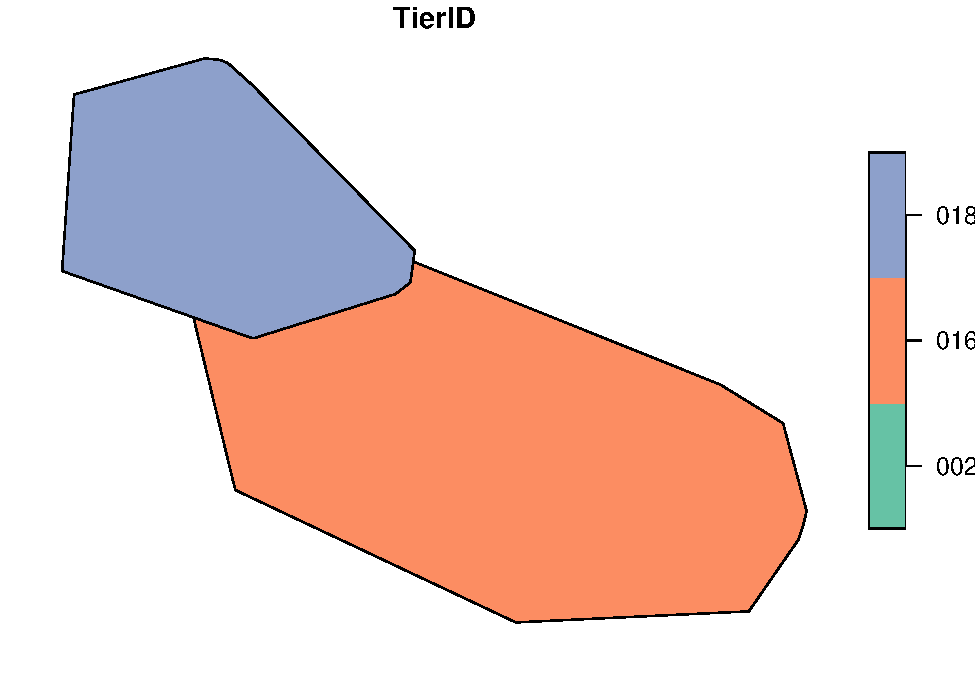
\includegraphics{_main_files/figure-latex/unnamed-chunk-19-1.pdf}

But since we use \texttt{ggplot} extensively, try and plot the object
\texttt{mcp} with \texttt{ggplot}. Hint: Since you installed the newest
version from github, you now use the function \texttt{geom\_sf()} to add
an \texttt{sf} object.

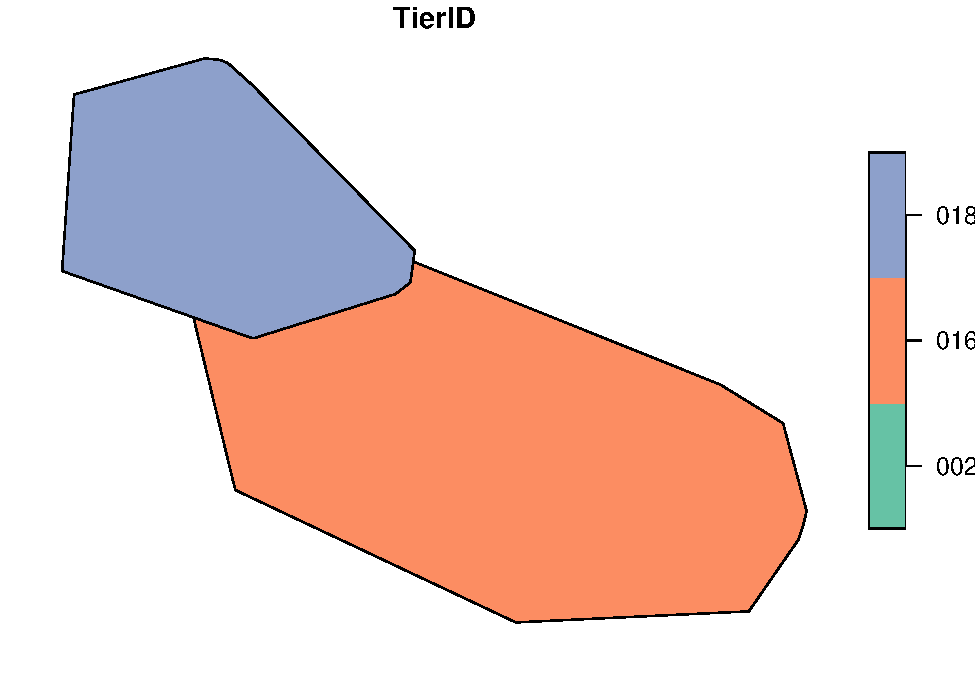
\includegraphics{_main_files/figure-latex/unnamed-chunk-20-1.pdf}

Note:

\begin{itemize}
\tightlist
\item
  \texttt{ggplot} refuses to use our specified CRS, so we need to force
  this by specifying \texttt{coord\_sf()}
\item
  Oddly, it is not sufficient to specify the \texttt{crs\ =} wit hin
  \texttt{coord\_sf()}, we need to pass our EPSG code to
  \texttt{datum\ =}.
\item
  You can change the plot style by making adjustments within
  \texttt{theme()} I recommend the following adjustments:
\end{itemize}

\begin{Shaded}
\begin{Highlighting}[]
\KeywordTok{theme}\NormalTok{(}
  \DataTypeTok{legend.position =} \StringTok{"none"}\NormalTok{,}
  \DataTypeTok{panel.grid.major =} \KeywordTok{element_line}\NormalTok{(}\DataTypeTok{colour =} \StringTok{"transparent"}\NormalTok{),}
  \DataTypeTok{panel.background =} \KeywordTok{element_rect}\NormalTok{(}\DataTypeTok{fill =} \StringTok{"transparent"}\NormalTok{),}
  \DataTypeTok{axis.title =} \KeywordTok{element_blank}\NormalTok{(),}
  \DataTypeTok{axis.text =} \KeywordTok{element_blank}\NormalTok{(),}
  \DataTypeTok{axis.ticks =} \KeywordTok{element_blank}\NormalTok{()}
  \NormalTok{)}
\end{Highlighting}
\end{Shaded}

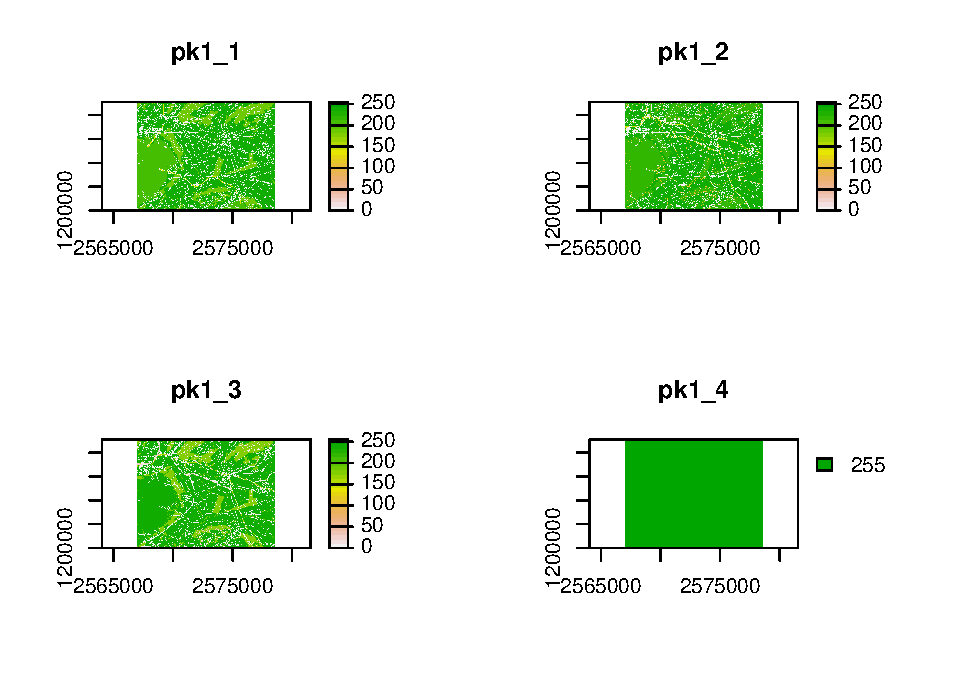
\includegraphics{_main_files/figure-latex/unnamed-chunk-22-1.pdf}

\subsection{Task 6: Adding a background
map}\label{task-6-adding-a-background-map}

In order to add a background map to our plot, we will need to load two
additional libraries: \texttt{raster} to load raster files and
\texttt{ggspatial} to plot raster files in \texttt{ggplot}. Load these
libraries now, and import the file \texttt{pk100\_BE\_2056.tif}
(available on moodle) using the function \texttt{brick()}. Add the newly
created \texttt{RasterBrick} object to ggplot using the function
\texttt{geom\_spraster\_rgb()}.

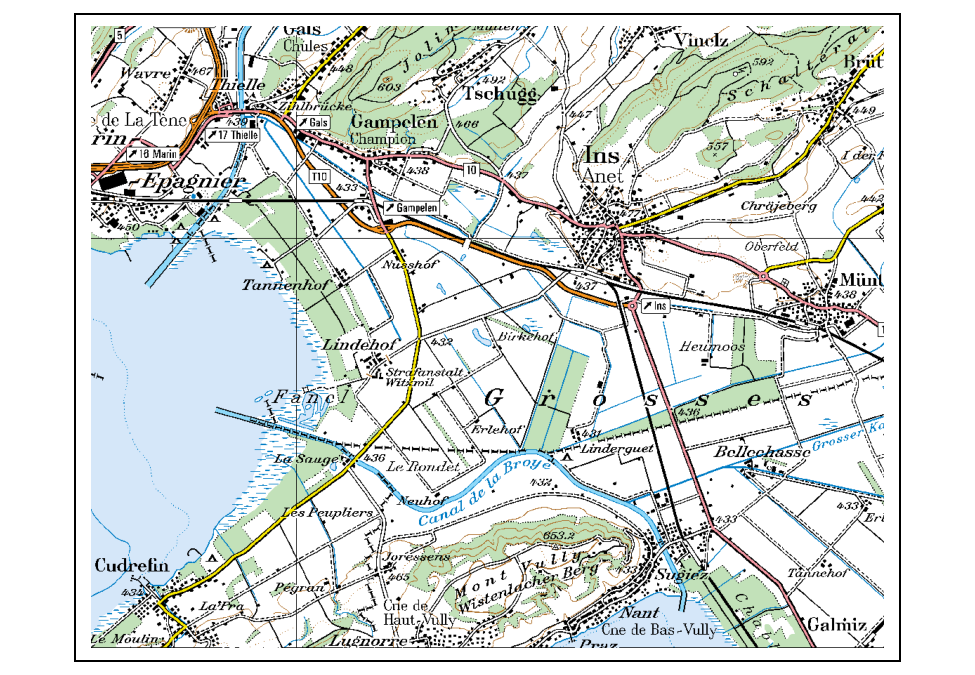
\includegraphics{_main_files/figure-latex/unnamed-chunk-23-1.pdf}

\chapter{Exercise 2}\label{exercise-2}

\section{Learning Outcomes}\label{learning-outcomes}

\section{Prerequisites}\label{prerequisites-1}

Readings Skills from ``R for Data Science'' (Wickham and Grolemund
2017):

\begin{itemize}
\tightlist
\item
  RS2.1 Chap3 Data Transformation with \texttt{dplyr} (31p, 43-76)
\item
  RS2.2 Chap10 Relational data with \texttt{dplyr} (21p, 171-193)
\item
  RS2.3 Chap14 Pipes with \texttt{magrittr} (6p, 261-268)
\end{itemize}

Readings Theory

\begin{itemize}
\tightlist
\item
  R2.1 Laube and Purves (2011): How fast is a cow? cross - scale
  analysis of movement data.
\end{itemize}

\section{Preperation}\label{preperation-1}

Open your R Project from last week. Load all libraries and run the
script to import and clean your data.

\begin{Shaded}
\begin{Highlighting}[]

\NormalTok{devtools::}\KeywordTok{install_git}\NormalTok{(}\StringTok{"https://github.engineering.zhaw.ch/PatternsTrendsEnvironmentalData/CMAtools.git"}\NormalTok{)}
\end{Highlighting}
\end{Shaded}

\section{Demo Tidyverse}\label{demo-tidyverse}

Depending on your knowledge of \texttt{R}, getting an overview of the
data we imported last week might have been quite a challenge.
Surprisingly enough, importing, cleaning and exploring your data can be
the most challenging, time consuming part of a project. RStudio and the
tidyverse offer many helpful tools to make this part easier (and more
fun). You have read chapters on \texttt{dplyr} and \texttt{magrittr} as
a preparation for this Exercise. Before we start with the Exercise
however, this demo illustrates a simple approach offered by tidyverse
which is applicable to sf-objects.

Assume we want to calculate the timelag in between subsequent positions.
To achieve this we can use the function \texttt{difftime()} combined
with \texttt{lead()} from \texttt{dplyr}. Let's look at these functions
one by one.

\subsection{\texorpdfstring{\texttt{difftime}}{difftime}}\label{difftime}

\texttt{difftime} takes two \texttt{POSIXct} values.

\begin{Shaded}
\begin{Highlighting}[]
\NormalTok{now <-}\StringTok{ }\KeywordTok{Sys.time}\NormalTok{()}

\NormalTok{later <-}\StringTok{ }\NormalTok{now +}\StringTok{ }\DecValTok{10000}

\NormalTok{time_difference <-}\StringTok{ }\KeywordTok{difftime}\NormalTok{(later,now)}
\end{Highlighting}
\end{Shaded}

You can also specify the unit of the output

\begin{Shaded}
\begin{Highlighting}[]
\NormalTok{time_difference <-}\StringTok{ }\KeywordTok{difftime}\NormalTok{(later,now,}\DataTypeTok{units =} \StringTok{"mins"}\NormalTok{)}
\end{Highlighting}
\end{Shaded}

\texttt{difftime} returns an object of the Class \texttt{difftime}.
However in our case, numeric values would be more handy than the Class
\texttt{difftime}. So we'll wrap the command in \texttt{as.numeric()}:

\begin{Shaded}
\begin{Highlighting}[]
\KeywordTok{str}\NormalTok{(time_difference)}
\NormalTok{## Class 'difftime'  atomic [1:1] 167}
\NormalTok{##   ..- attr(*, "units")= chr "mins"}
\end{Highlighting}
\end{Shaded}

\begin{Shaded}
\begin{Highlighting}[]
\NormalTok{time_difference <-}\StringTok{ }\KeywordTok{as.numeric}\NormalTok{(}\KeywordTok{difftime}\NormalTok{(later,now,}\DataTypeTok{units =} \StringTok{"mins"}\NormalTok{))}

\KeywordTok{str}\NormalTok{(time_difference)}
\NormalTok{##  num 167}
\end{Highlighting}
\end{Shaded}

\subsection{\texorpdfstring{\texttt{lead()} /
\texttt{lag()}}{lead() / lag()}}\label{lead-lag}

\texttt{lead()} and \texttt{lag()} return a vector of the same length as
the input, just offset by a specific number of values (default is 1).
Consider the following sequence:

\begin{Shaded}
\begin{Highlighting}[]
\NormalTok{numbers <-}\StringTok{ }\DecValTok{1}\NormalTok{:}\DecValTok{10}

\NormalTok{numbers}
\NormalTok{##  [1]  1  2  3  4  5  6  7  8  9 10}
\end{Highlighting}
\end{Shaded}

We can now run \texttt{lead()} and \texttt{lag()} on this sequence to
illustrate the output. \texttt{n\ =} specifies the offset,
\texttt{default\ =} specifies the default value used to ``fill'' the
vector.

\begin{Shaded}
\begin{Highlighting}[]
\KeywordTok{lead}\NormalTok{(numbers)}
\NormalTok{##  [1]  2  3  4  5  6  7  8  9 10 NA}

\KeywordTok{lead}\NormalTok{(numbers,}\DataTypeTok{n =} \DecValTok{2}\NormalTok{)}
\NormalTok{##  [1]  3  4  5  6  7  8  9 10 NA NA}

\KeywordTok{lag}\NormalTok{(numbers)}
\NormalTok{##  [1] NA  1  2  3  4  5  6  7  8  9}

\KeywordTok{lag}\NormalTok{(numbers,}\DataTypeTok{n =} \DecValTok{5}\NormalTok{)}
\NormalTok{##  [1] NA NA NA NA NA  1  2  3  4  5}

\KeywordTok{lag}\NormalTok{(numbers,}\DataTypeTok{n =} \DecValTok{5}\NormalTok{, }\DataTypeTok{default =} \DecValTok{0}\NormalTok{)}
\NormalTok{##  [1] 0 0 0 0 0 1 2 3 4 5}
\end{Highlighting}
\end{Shaded}

This helps us performing operations on subsequent values in a vector (or
rows in a table)

\subsection{\texorpdfstring{\texttt{mutate()}}{mutate()}}\label{mutate}

Using the above functions (\texttt{difftime()} and \texttt{lead()}), we
can calculate the time difference between subsequent positions:

\begin{Shaded}
\begin{Highlighting}[]
\NormalTok{wildschwein_BE$timelag  <-}\StringTok{ }\KeywordTok{as.numeric}\NormalTok{(}\KeywordTok{difftime}\NormalTok{(}\KeywordTok{lead}\NormalTok{(wildschwein_BE$DatetimeUTC),wildschwein_BE$DatetimeUTC,}\DataTypeTok{units =} \StringTok{"secs"}\NormalTok{))}
\end{Highlighting}
\end{Shaded}

We mention \texttt{wildschwein\_BE} three times in this function, which
is why we can use \texttt{mutate()}:

\begin{Shaded}
\begin{Highlighting}[]
\NormalTok{wildschwein_BE <-}\StringTok{ }\KeywordTok{mutate}\NormalTok{(wildschwein_BE,}\DataTypeTok{timelag =} \KeywordTok{as.numeric}\NormalTok{(}\KeywordTok{difftime}\NormalTok{(}\KeywordTok{lead}\NormalTok{(DatetimeUTC),DatetimeUTC,}\DataTypeTok{units =} \StringTok{"secs"}\NormalTok{)))}
\end{Highlighting}
\end{Shaded}

Now let's have a look at this vector:

\begin{Shaded}
\begin{Highlighting}[]
\KeywordTok{summary}\NormalTok{(wildschwein_BE$timelag)}
\NormalTok{##      Min.   1st Qu.    Median      Mean   3rd Qu.      Max.      NA's }
\NormalTok{## -65155503       895       900       259       907  49579199         1}
\end{Highlighting}
\end{Shaded}

These values don't make much sense: some are negative (which should not
be the case) and some are very high (which would indicate large data
gaps and should not be the case either). The reason for this result is
that we did not consider that \texttt{timelag} should just be calculated
between subsequent rows \emph{of the same individual}. We can implement
this by using \texttt{group\_by()} (just as if calculating the convex
hull last week).

\begin{Shaded}
\begin{Highlighting}[]
\NormalTok{wildschwein_BE <-}\StringTok{ }\KeywordTok{group_by}\NormalTok{(wildschwein_BE,TierID)}
\end{Highlighting}
\end{Shaded}

After adding this grouping variable, calculating the timelag
automatically accounts for the individual trajectories.

\begin{Shaded}
\begin{Highlighting}[]
\NormalTok{wildschwein_BE <-}\StringTok{ }\KeywordTok{mutate}\NormalTok{(wildschwein_BE,}\DataTypeTok{timelag =} \KeywordTok{as.numeric}\NormalTok{(}\KeywordTok{difftime}\NormalTok{(}\KeywordTok{lead}\NormalTok{(DatetimeUTC),DatetimeUTC,}\DataTypeTok{units =} \StringTok{"secs"}\NormalTok{)))}

\KeywordTok{summary}\NormalTok{(wildschwein_BE$timelag)}
\NormalTok{##    Min. 1st Qu.  Median    Mean 3rd Qu.    Max.    NA's }
\NormalTok{##      12     895     900    1203     907  108023      10}
\end{Highlighting}
\end{Shaded}

Summary returned the metrics over all individuals. If we want to
summarise our data and get metrics \emph{per animal}, we can use the
\texttt{dplyr} function \texttt{summarise()}. In contrast to
\texttt{mutate()}, which just adds a new column to the dataset,
\texttt{summarise()} ``collapses'' the data to one row per individual
(specified by \texttt{group\_by}).

\begin{Shaded}
\begin{Highlighting}[]
\KeywordTok{summarise}\NormalTok{(wildschwein_BE, }\DataTypeTok{mean =} \KeywordTok{mean}\NormalTok{(timelag, }\DataTypeTok{na.rm =} \NormalTok{T))}
\end{Highlighting}
\end{Shaded}

The above operation works fine on normal \texttt{data.frames}, but since
\texttt{wildschwein\_BE} is also an \texttt{sf} object,
\texttt{summarise} actually merges all the points to a multipoint
geometry, which takes a long time to calculate. In order to prevent
this, we can wrap the \texttt{sf} object in \texttt{as.data.frame} which
removes the spatial attribute. Regrettably, it also removes the
\texttt{group\_by} variable, which we need to set again. The command
therefore goes like:

\begin{Shaded}
\begin{Highlighting}[]
\KeywordTok{summarise}\NormalTok{(}\KeywordTok{group_by}\NormalTok{(}\KeywordTok{as.data.frame}\NormalTok{(wildschwein_BE),TierID), }\DataTypeTok{mean_timelag =} \KeywordTok{mean}\NormalTok{(timelag, }\DataTypeTok{na.rm =} \NormalTok{T))}
\NormalTok{## # A tibble: 10 x 2}
\NormalTok{##    TierID mean_timelag}
\NormalTok{##    <chr>         <dbl>}
\NormalTok{##  1 001A          1661.}
\NormalTok{##  2 001B           900.}
\NormalTok{##  3 002A          1286.}
\NormalTok{##  4 005A          1825.}
\NormalTok{##  5 010A           980.}
\NormalTok{##  6 010B          1607.}
\NormalTok{##  7 010C           694.}
\NormalTok{##  8 011A          2736.}
\NormalTok{##  9 016A          1412.}
\NormalTok{## 10 018A          1599.}
\end{Highlighting}
\end{Shaded}

This code is hard to read, since it has so many nested functions which
need to be read from the inside out. In order to make code readable in a
more human-friendly way, we can use the piping command
\texttt{\%\textgreater{}\%} from \texttt{magrittr}, which is included in
\texttt{dplyr} and the \texttt{tidyverse}. The above code then looks
like this:

\begin{Shaded}
\begin{Highlighting}[]
\NormalTok{wildschwein_BE %>%}\StringTok{                     }\CommentTok{# Take wildschwein_BE...}
\StringTok{  }\KeywordTok{as.data.frame}\NormalTok{() %>%}\StringTok{                  }\CommentTok{# ...convert it to a data.frame...}
\StringTok{  }\KeywordTok{group_by}\NormalTok{(TierID) %>%}\StringTok{                 }\CommentTok{# ...group it by TierID}
\StringTok{  }\KeywordTok{summarise}\NormalTok{(                           }\CommentTok{# Summarise the data...}
    \DataTypeTok{mean_timelag =} \KeywordTok{mean}\NormalTok{(timelag,}\DataTypeTok{na.rm =} \NormalTok{T) }\CommentTok{# ...by calculating the mean timelag}
  \NormalTok{)}
\NormalTok{## # A tibble: 10 x 2}
\NormalTok{##    TierID mean_timelag}
\NormalTok{##    <chr>         <dbl>}
\NormalTok{##  1 001A          1661.}
\NormalTok{##  2 001B           900.}
\NormalTok{##  3 002A          1286.}
\NormalTok{##  4 005A          1825.}
\NormalTok{##  5 010A           980.}
\NormalTok{##  6 010B          1607.}
\NormalTok{##  7 010C           694.}
\NormalTok{##  8 011A          2736.}
\NormalTok{##  9 016A          1412.}
\NormalTok{## 10 018A          1599.}
\end{Highlighting}
\end{Shaded}

\section{Tasks and Inputs}\label{tasks-and-inputs-1}

\subsection{Task 1: Getting an
Overview}\label{task-1-getting-an-overview}

First, inspect your data in more detail. Try to answer the following
questions:

\begin{itemize}
\tightlist
\item
  How many individuals were tracked?
\item
  How long were the individual tracked? Are there gaps?
\item
  Were all individuals tracked concurrently or sequentially?
\item
  What is the temporal sampling interval between the locations?
\end{itemize}

Here are some exemplary visualisation you could produce to answer these
questions. Can you now answer the above questions?
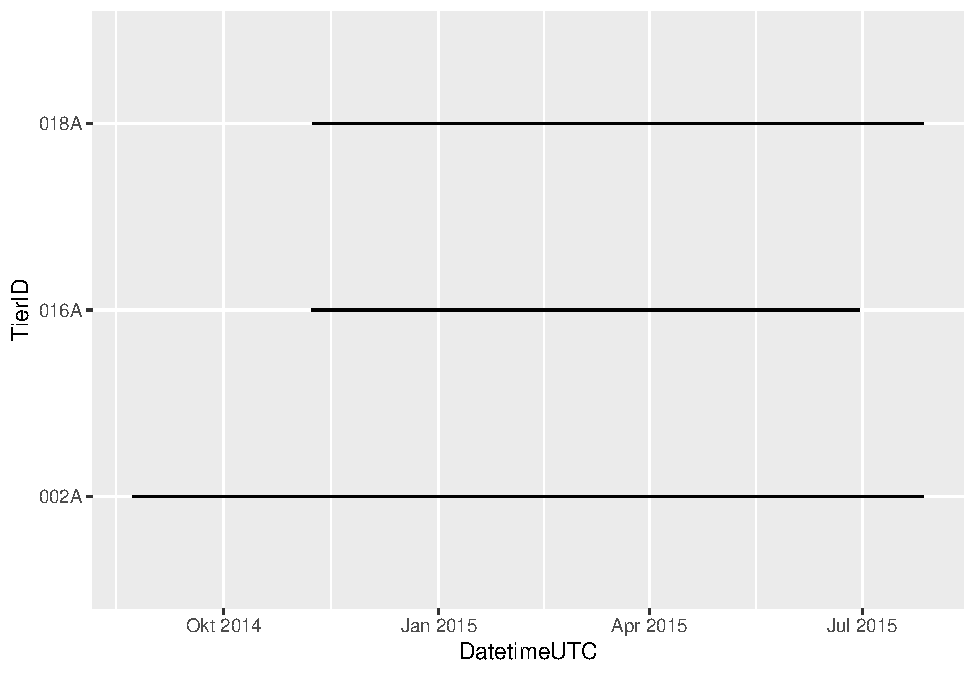
\includegraphics{_main_files/figure-latex/unnamed-chunk-45-1.pdf}
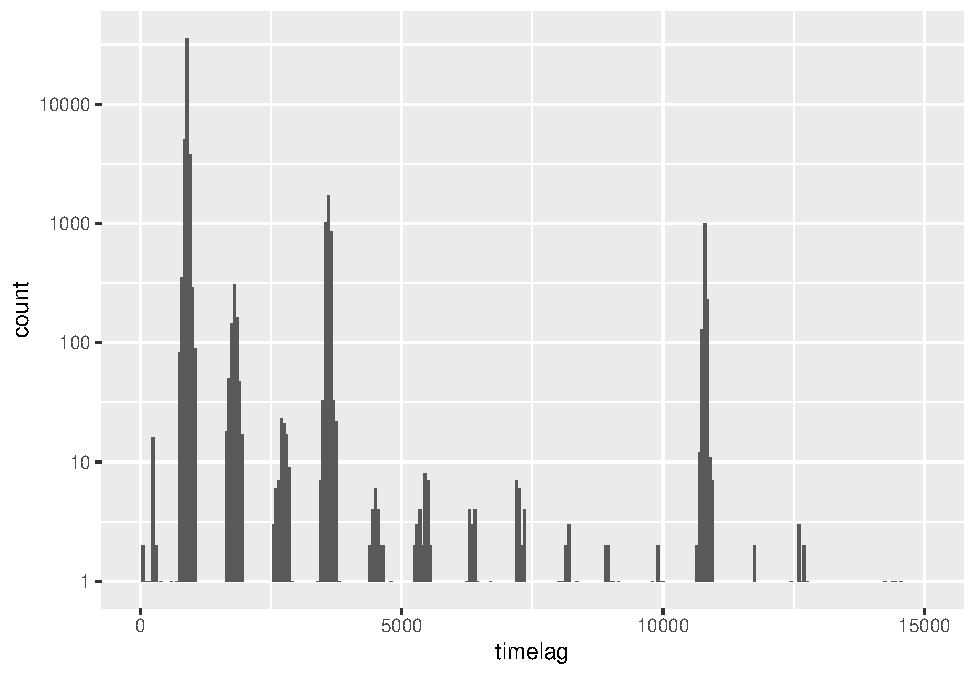
\includegraphics{_main_files/figure-latex/unnamed-chunk-45-2.pdf}
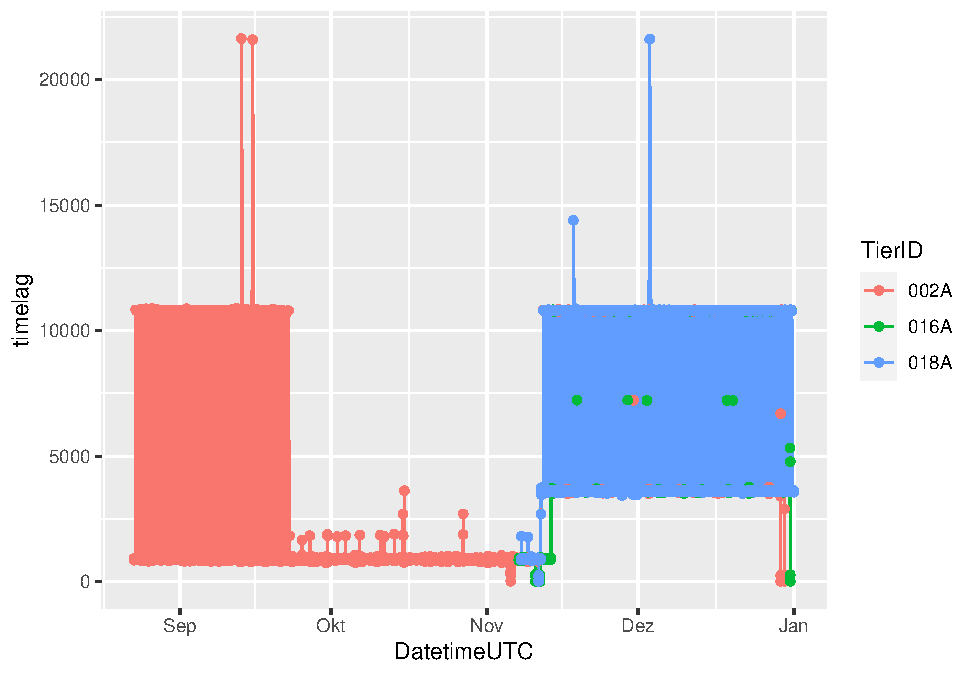
\includegraphics{_main_files/figure-latex/unnamed-chunk-45-3.pdf}
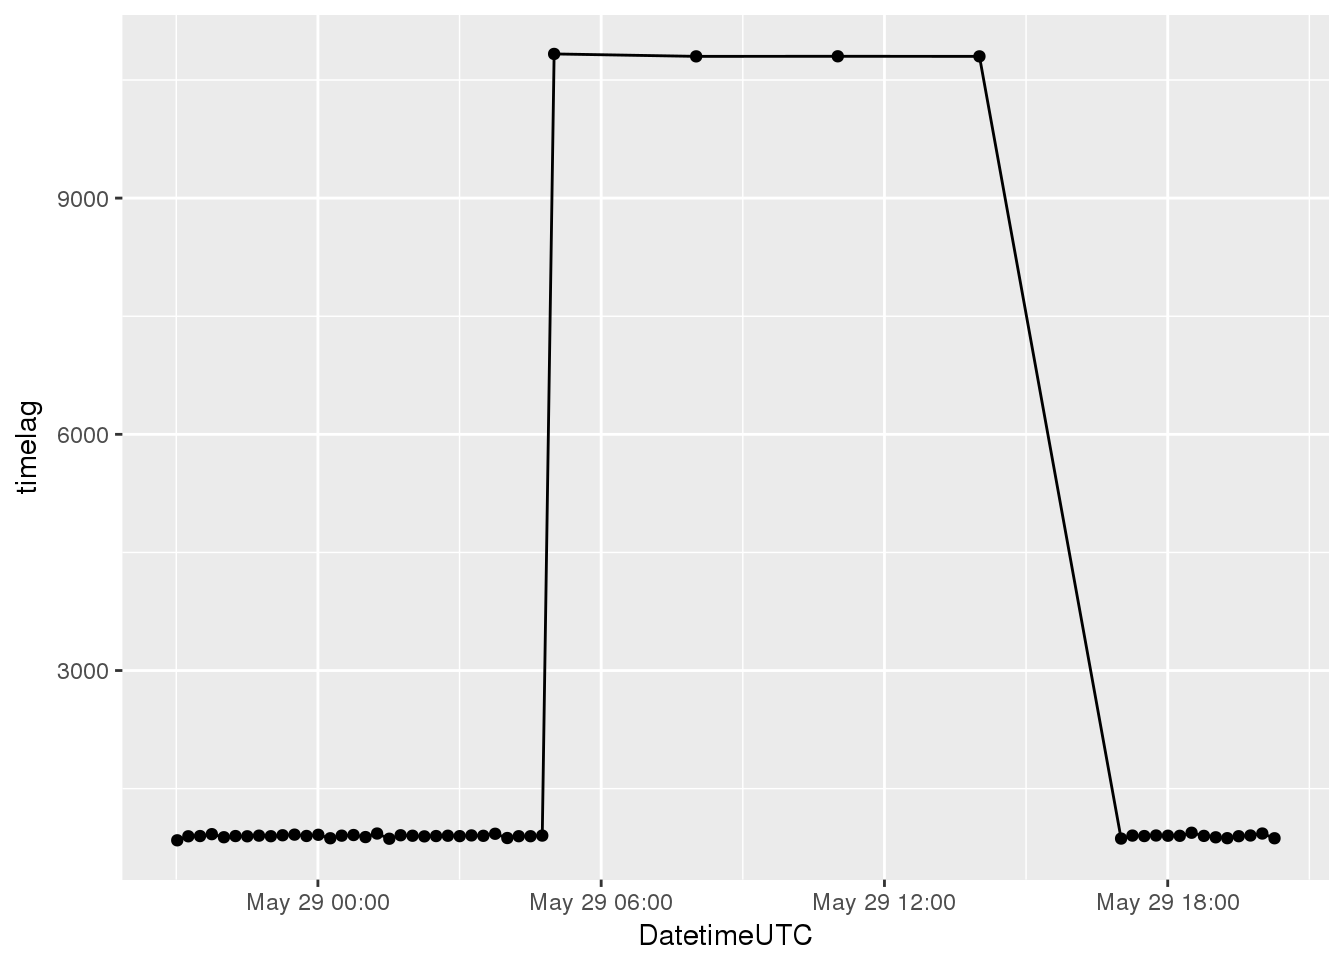
\includegraphics{_main_files/figure-latex/unnamed-chunk-45-4.pdf}

\subsection{\texorpdfstring{Input: \texttt{cut()} vector by
intervals}{Input: cut() vector by intervals}}\label{input-cut-vector-by-intervals}

For the next Task, we will need a function to split a continuous
variable into specific intervals. For this, the function
\texttt{cut()}is very handy. Let's introduce this function with a quick
example. Assume we have a series of number that represent the ages of
ten different people.

\begin{Shaded}
\begin{Highlighting}[]
\NormalTok{ages <-}\StringTok{ }\KeywordTok{c}\NormalTok{(}\DecValTok{20}\NormalTok{,}\DecValTok{25}\NormalTok{,}\DecValTok{18}\NormalTok{,}\DecValTok{13}\NormalTok{,}\DecValTok{53}\NormalTok{,}\DecValTok{50}\NormalTok{,}\DecValTok{23}\NormalTok{,}\DecValTok{43}\NormalTok{,}\DecValTok{68}\NormalTok{,}\DecValTok{40}\NormalTok{)}
\end{Highlighting}
\end{Shaded}

Let's say we want to split this into equal intervals of 10 years.

\begin{Shaded}
\begin{Highlighting}[]
\NormalTok{breaks <-}\StringTok{ }\KeywordTok{seq}\NormalTok{(}\DecValTok{0}\NormalTok{,}\DecValTok{50}\NormalTok{,}\DecValTok{10}\NormalTok{)}

\KeywordTok{cut}\NormalTok{(ages,}\DataTypeTok{breaks =} \NormalTok{breaks)}
\NormalTok{##  [1] (10,20] (20,30] (10,20] (10,20] <NA>    (40,50] (20,30] (40,50]}
\NormalTok{##  [9] <NA>    (30,40]}
\NormalTok{## Levels: (0,10] (10,20] (20,30] (30,40] (40,50]}
\end{Highlighting}
\end{Shaded}

Note:

\begin{itemize}
\tightlist
\item
  If a number does not fit within an interval defined by
  \texttt{breaks\ =}, \texttt{cut()} will return \texttt{NA} (as for
  example for the fifth element \texttt{53}).
\item
  The default \texttt{labels} with \texttt{(} and \texttt{{]}} might
  seem a little ugly and puzzling at first, but in fact they are
  \href{https://en.wikipedia.org/wiki/Interval_\%28mathematics\%29\#Notations_for_intervals}{a
  standard form of notating intervals in mathematics}.
\item
  If you don't like \texttt{(} and \texttt{{]}}, you can:
\item
  specify your own labels with the argument \texttt{labels\ =} \emph{or}
\item
  use the the function \texttt{labels\_nice} we provide with the
  \texttt{CMAtools}-package
\item
  Four thresholds (i.e. \texttt{breaks}) return three intervals (i.e.
  \texttt{lables}), as shown below.
\end{itemize}

\begin{Shaded}
\begin{Highlighting}[]

\NormalTok{breaks <-}\StringTok{ }\KeywordTok{c}\NormalTok{(}\DecValTok{0}\NormalTok{,}\DecValTok{30}\NormalTok{,}\DecValTok{60}\NormalTok{,}\DecValTok{100}\NormalTok{)}

\KeywordTok{cut}\NormalTok{(ages, }\DataTypeTok{breaks =} \NormalTok{breaks, }\DataTypeTok{labels =} \KeywordTok{c}\NormalTok{(}\StringTok{"young"}\NormalTok{,}\StringTok{"middle aged"}\NormalTok{,}\StringTok{"old"}\NormalTok{))}
\NormalTok{##  [1] young       young       young       young       middle aged}
\NormalTok{##  [6] middle aged young       middle aged old         middle aged}
\NormalTok{## Levels: young middle aged old}

\KeywordTok{cut}\NormalTok{(ages, }\DataTypeTok{breaks =} \NormalTok{breaks, }\DataTypeTok{labels =} \NormalTok{CMAtools::}\KeywordTok{labels_nice}\NormalTok{(breaks))}
\NormalTok{##  [1] 0-30   0-30   0-30   0-30   30-60  30-60  0-30   30-60  60-100 30-60 }
\NormalTok{## Levels: 0-30 30-60 60-100}
\end{Highlighting}
\end{Shaded}

\subsection{Task 2: Making groups by sampling
Interval}\label{task-2-making-groups-by-sampling-interval}

Now that we've established that we have different sampling intervals
(Task 1), we have to segment our trajectories in such a way, that we can
perform further analysis during specific sampling intervals only. If we
measure speed, or turning angles, we have to be very clear on what
temporal (an thus spatial) scale or granularity we are performing this
analysis.

We therefore have to define thresholds to group segments with a similar
sampling interval. Explore the dataset in more detail (e.g.~using
histograms at different scales), and choose reasonable threshold values
to group the trajectories into different sampling intervals.

Note:

\begin{itemize}
\tightlist
\item
  It might make more sense to choose narrow intervals at shorter time
  lags and wider intervals at longer time lags.
\item
  Store the interval names in a new column named \texttt{samplingInt}
\end{itemize}

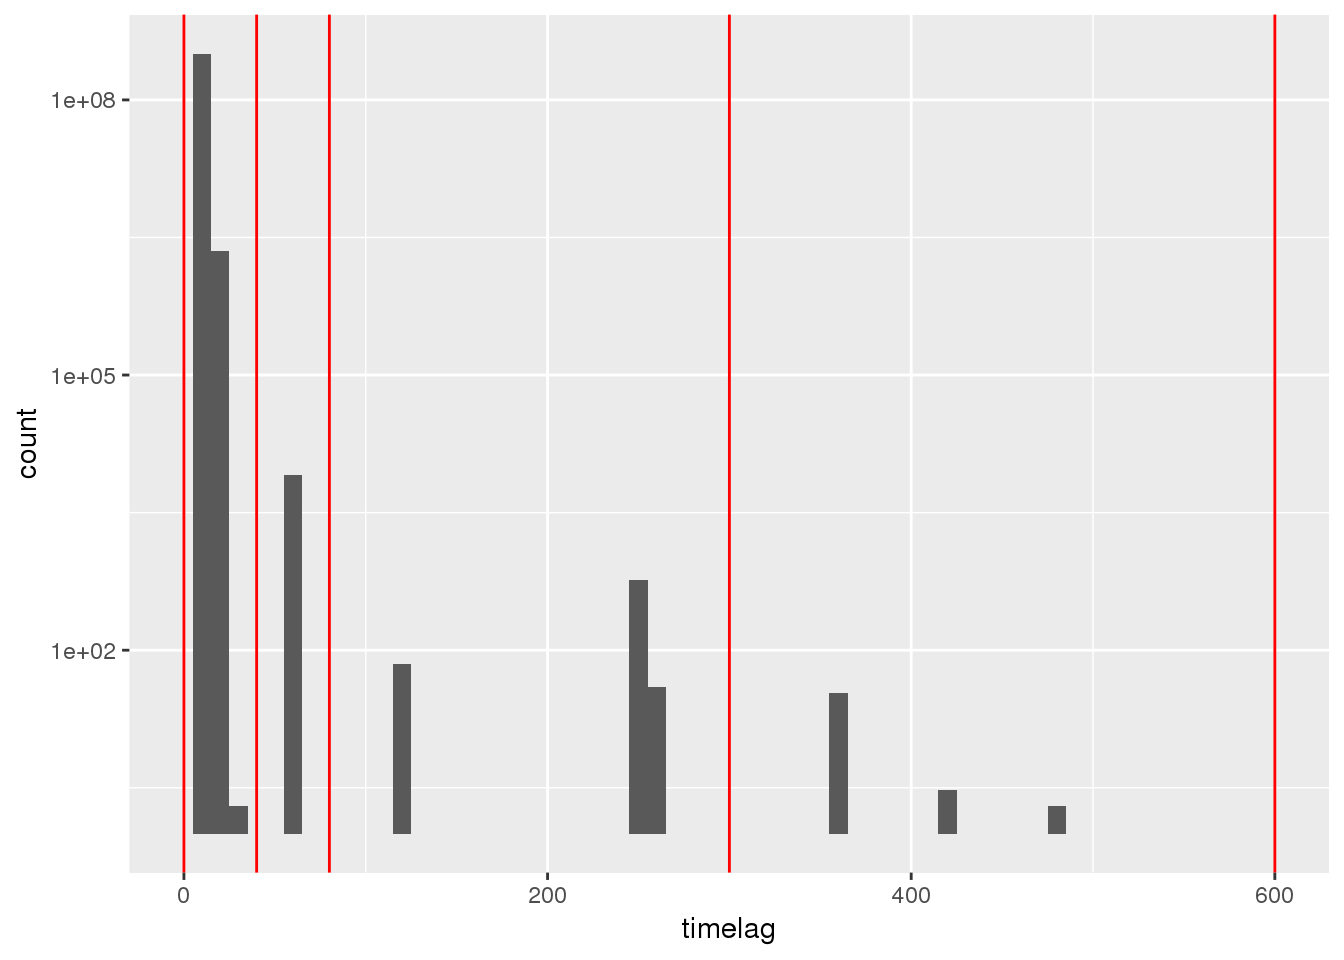
\includegraphics{_main_files/figure-latex/unnamed-chunk-50-1.pdf}
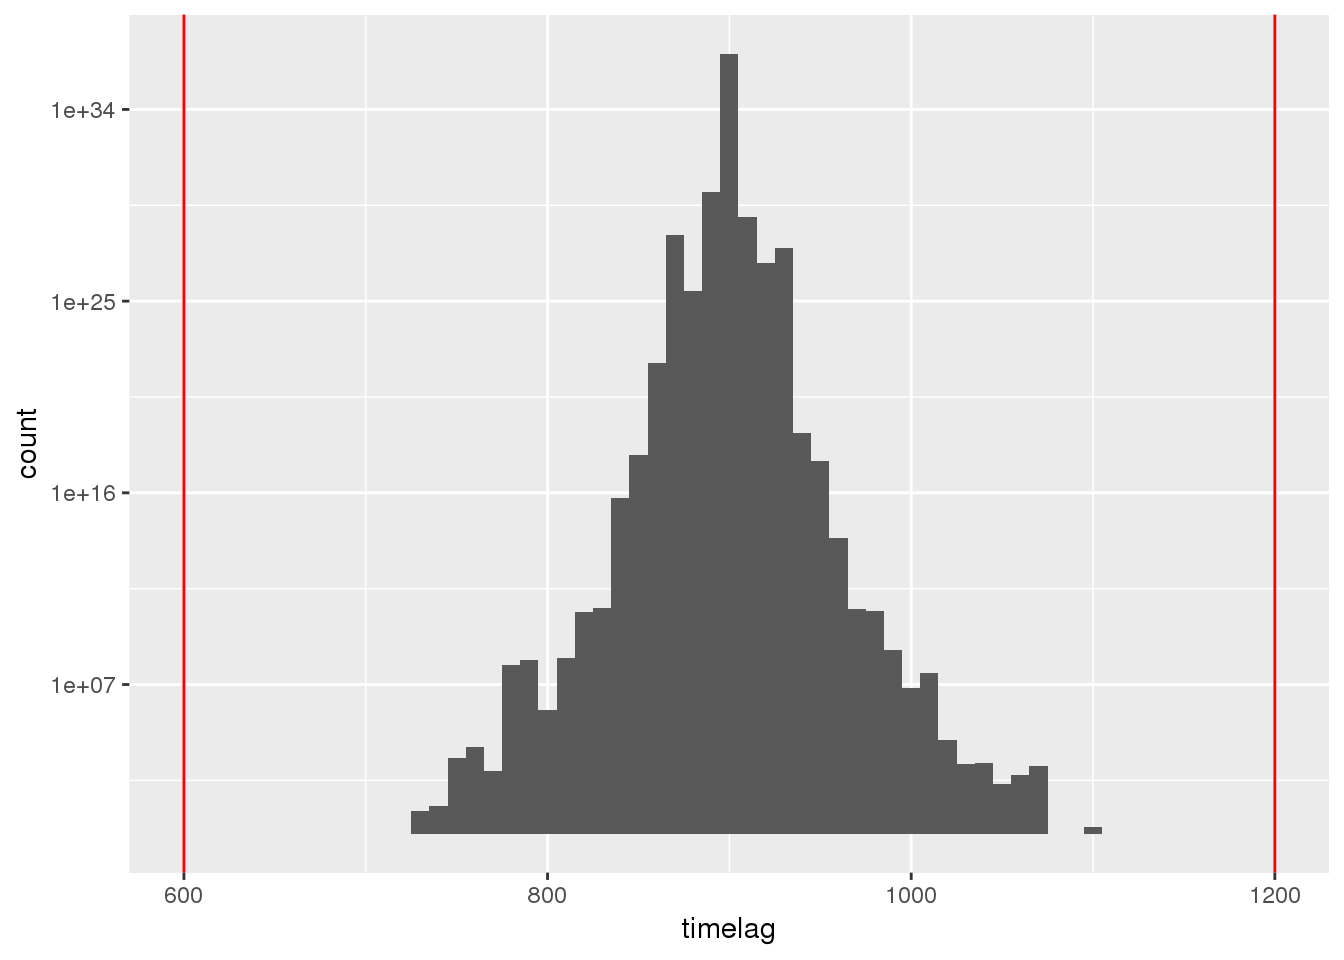
\includegraphics{_main_files/figure-latex/unnamed-chunk-50-2.pdf}
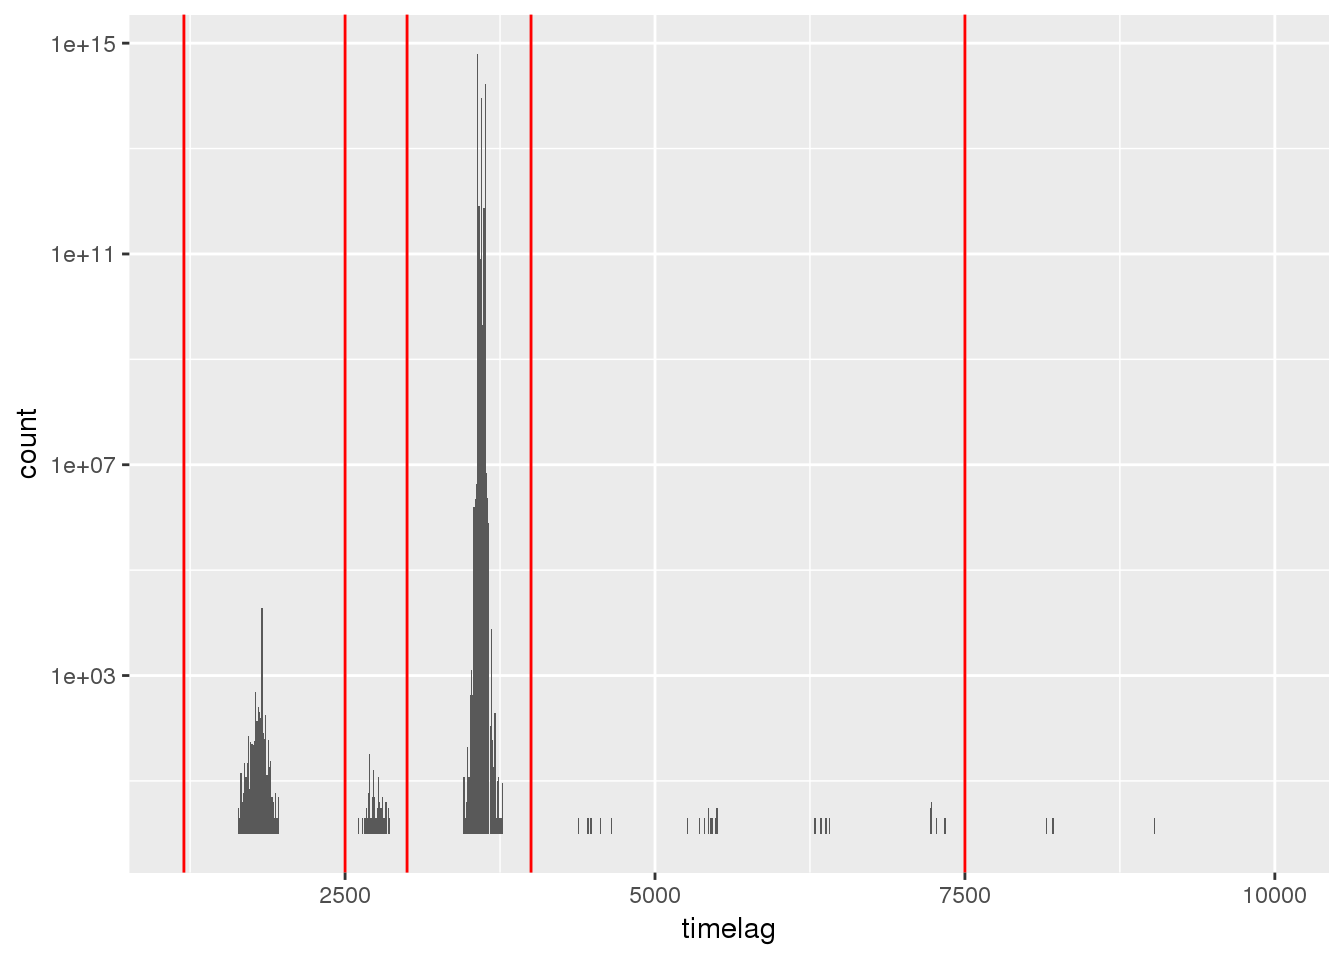
\includegraphics{_main_files/figure-latex/unnamed-chunk-50-3.pdf}
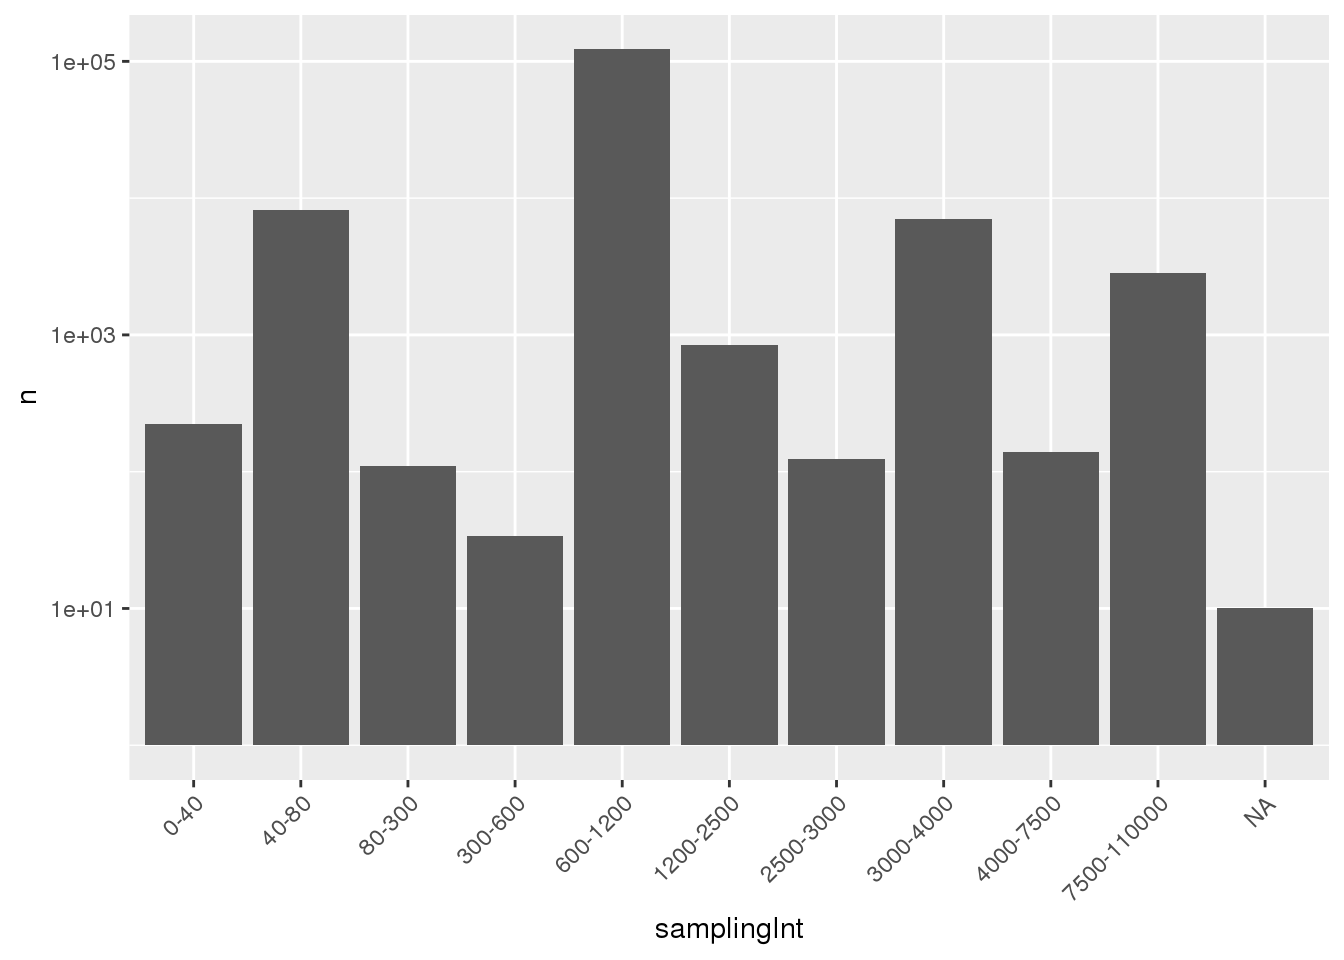
\includegraphics{_main_files/figure-latex/unnamed-chunk-50-4.pdf}

\subsection{Input: Geometry as columns}\label{input-geometry-as-columns}

Last week, we transformed our data from a \texttt{data.frame} to an
\texttt{sf} object. This turned our \texttt{Lat}/\texttt{Long} Columns
into a single geometry (list) column. While this is very handy for many
spatial operations, accessing the coordinates directly becomes
difficult. We therefore suggest storing the information twice, once as a
geometry and once as a numeric value. We did this for the values in
\texttt{WGS84}, but not yet for \texttt{CH1903+\ LV95}.

\begin{Shaded}
\begin{Highlighting}[]

\NormalTok{wildschwein_BE}
\NormalTok{## Simple feature collection with 141763 features and 8 fields}
\NormalTok{## geometry type:  POINT}
\NormalTok{## dimension:      XY}
\NormalTok{## bbox:           xmin: 2568153 ymin: 1201483 xmax: 2577023 ymax: 1207609}
\NormalTok{## epsg (SRID):    2056}
\NormalTok{## proj4string:    +proj=somerc +lat_0=46.95240555555556 +lon_0=7.439583333333333 +k_0=1 +x_0=2600000 +y_0=1200000 +ellps=bessel +towgs84=674.374,15.056,405.346,0,0,0,0 +units=m +no_defs}
\NormalTok{## # A tibble: 141,763 x 9}
\NormalTok{## # Groups:   TierID [10]}
\NormalTok{##    TierID TierName CollarID DatetimeUTC           Lat  Long timelag}
\NormalTok{##    <chr>  <chr>       <int> <dttm>              <dbl> <dbl>   <dbl>}
\NormalTok{##  1 001A   Ueli        12272 2014-05-28 21:01:14  47.0  7.05    844.}
\NormalTok{##  2 001A   Ueli        12272 2014-05-28 21:15:18  47.0  7.05    895.}
\NormalTok{##  3 001A   Ueli        12272 2014-05-28 21:30:13  47.0  7.05    898.}
\NormalTok{##  4 001A   Ueli        12272 2014-05-28 21:45:11  47.0  7.05    922.}
\NormalTok{##  5 001A   Ueli        12272 2014-05-28 22:00:33  47.0  7.05    883.}
\NormalTok{##  6 001A   Ueli        12272 2014-05-28 22:15:16  47.0  7.05    898.}
\NormalTok{##  7 001A   Ueli        12272 2014-05-28 22:30:14  47.0  7.05    895.}
\NormalTok{##  8 001A   Ueli        12272 2014-05-28 22:45:09  47.0  7.05    903.}
\NormalTok{##  9 001A   Ueli        12272 2014-05-28 23:00:12  47.0  7.05    896.}
\NormalTok{## 10 001A   Ueli        12272 2014-05-28 23:15:08  47.0  7.05    908.}
\NormalTok{## # ... with 141,753 more rows, and 2 more variables: samplingInt <fct>,}
\NormalTok{## #   geometry <POINT [m]>}
\end{Highlighting}
\end{Shaded}

Let's do the same for the \texttt{CH1903+\ LV95}-values, as we will need
the values in columns for our next task. First, we have to extract the
Coordinates using \texttt{st\_coordinates()}. We can store these values
in a new variable and display them:

\begin{Shaded}
\begin{Highlighting}[]
\CommentTok{# Store coordinates in a new variable}
\NormalTok{coordinates <-}\StringTok{ }\KeywordTok{st_coordinates}\NormalTok{(wildschwein_BE)}

\KeywordTok{head}\NormalTok{(coordinates)}
\NormalTok{##         X       Y}
\NormalTok{## 1 2570390 1204820}
\NormalTok{## 2 2570389 1204826}
\NormalTok{## 3 2570391 1204821}
\NormalTok{## 4 2570388 1204826}
\NormalTok{## 5 2570388 1204819}
\NormalTok{## 6 2570384 1204828}
\end{Highlighting}
\end{Shaded}

Note that that the column are named \texttt{X} and \texttt{Y}, while
\href{https://www.swisstopo.admin.ch/de/wissen-fakten/geodaesie-vermessung/neue-koordinaten.html}{\texttt{CH1903+\ LV95}}
names the Axes \texttt{E} and \texttt{N}: let's rename the columns
appropriately. After this, we can use \texttt{cbind()} to ``glue'' the
columns to our original \texttt{sf}-object.

\begin{Shaded}
\begin{Highlighting}[]
\KeywordTok{colnames}\NormalTok{(coordinates) <-}\StringTok{ }\KeywordTok{c}\NormalTok{(}\StringTok{"E"}\NormalTok{,}\StringTok{"N"}\NormalTok{)}

\NormalTok{wildschwein_BE <-}\StringTok{ }\KeywordTok{cbind}\NormalTok{(wildschwein_BE,coordinates)}
\end{Highlighting}
\end{Shaded}

\subsection{Task 3: Deriving movement parameters I: Euclidean Distance
and
Speed}\label{task-3-deriving-movement-parameters-i-euclidean-distance-and-speed}

In this task we will derive some additional movement parameters from our
trajectories. Note, so far our trajectories only consist of a list of
time-stamped spatial locations. So let's calculate the animal's speed
based on the distance and timelag in between two subsequent locations.

\begin{itemize}
\tightlist
\item
  If you're working with \texttt{dplyr}, you can add
  \texttt{samplingInt} to \texttt{group\_by()} (in addition to
  \texttt{TierID}) and so make sure you're not calculating speed across
  different sampling intervals.
\item
  You can use the function \texttt{euclid()} from the \texttt{CMAtools}
  package to calculate Euclidean distances between subsequent rows. Use
  ?euclid to see what the function expects and returns.
\item
  use \texttt{lead(E,1)} to address the the row \texttt{n+1}
\item
  make sure you're clear in what unit you are measuring speed. Meters
  per second is a SI base unit, but might be unhandy for the speeds
  travelled by wild boar. Perhaps make two speed columns, one in meters
  per second and one in km per hour?
\end{itemize}

\subsection{Task 4}\label{task-4}

Laube and Purves (2011) analyse animal movement across different scales
(see below).

\begin{figure}[htbp]
\centering
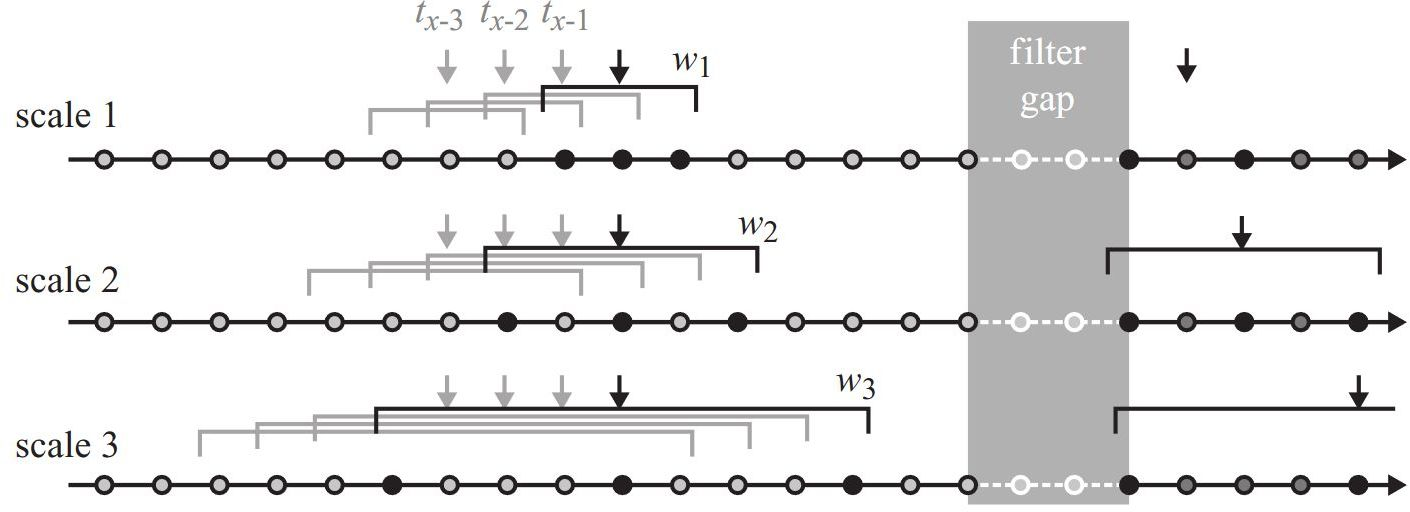
\includegraphics{02_Images/laube_2011_2.jpg}
\caption{Black points are used in calculation of movement parameters
(e.g.~speed) at a given termporal scale.}
\end{figure}

We will do the same for our data and will be working on a \emph{subset}
of our dataset. We will only need trajectories with a sampling interval
of around 60 seconds (\$\pm\$20 seconds). Filter your data accordingly
and save it to a new variable (we will use \texttt{wildschwein\_BE\_1}).
From this subset, take the first 100 positions for the following task.
If you like to stick to the \texttt{tidyverse} approach, you can use
\texttt{slice()} to subset the dataset by row number. Slice takes an
integer vector. Eg: \texttt{slice(dataset,\ 1:10)}, returns the first 10
rows of a dataset, \texttt{slice(dataset,\ c(1,5,10))} returns the
1\textsuperscript{st}, 5\textsuperscript{th} and 10\textsuperscript{th}
value of a dataset.

Now manually reduce the granularity of our sampling interval by
selecting samples every 3\textsuperscript{rd}, 6\textsuperscript{th} and
9\textsuperscript{th} minute.

\begin{itemize}
\tightlist
\item
  You can use \texttt{slice()} again for this task by providing an
  integer vector (with \texttt{seq()}) in the desired frequency
\item
  Save each resampled dataset in a new variable. We will use
  (\^{}wildschwein\_BE\_3\texttt{,}wildschwein\_BE\_6\texttt{and}wildschwein\_BE\_9`)
\end{itemize}

\texttt{timelag}, \texttt{steplength} and \texttt{speed} now have to be
recalculated on the basis of the resampled data. Do so as we illustrated
in the Chapter \emph{Demo}.

Compare the speeds in a line plot and viualize the trajectories in a map
(see examples below). Interpret the line plot, what do the different
lines for the different temporal granularities tell you?

We've stored our location data in three different form in our dataset.
Once as a \texttt{geometry}, once as \texttt{E}/\texttt{N} and once as
\texttt{lat}/\texttt{long}. In our view, it is most practical to use the
\texttt{E}/\texttt{N} (integer) columns of our data to map them in this
task

\begin{itemize}
\tightlist
\item
  \texttt{geom\_sf()} does not plot lines, just points
\item
  Therefore, use \texttt{geom\_path()} \emph{and} \texttt{geom\_point()}
  rather than \texttt{geom\_sf()} within \texttt{ggplot}
\item
  In contrast to \texttt{geom\_sf()}, you have to explicitly specify the
  \texttt{x}/\texttt{y} columns (in our case \texttt{E}/\texttt{N}) with
  \texttt{geom\_path()}/\texttt{geom\_point()}
\item
  \texttt{geom\_line()} does not work when mapping trajectory data,
  since it connects the observations \emph{in order of the variable on
  the x axis}. \texttt{geom\_path()} connects the observations in the
  order in which they appear in the data
\end{itemize}

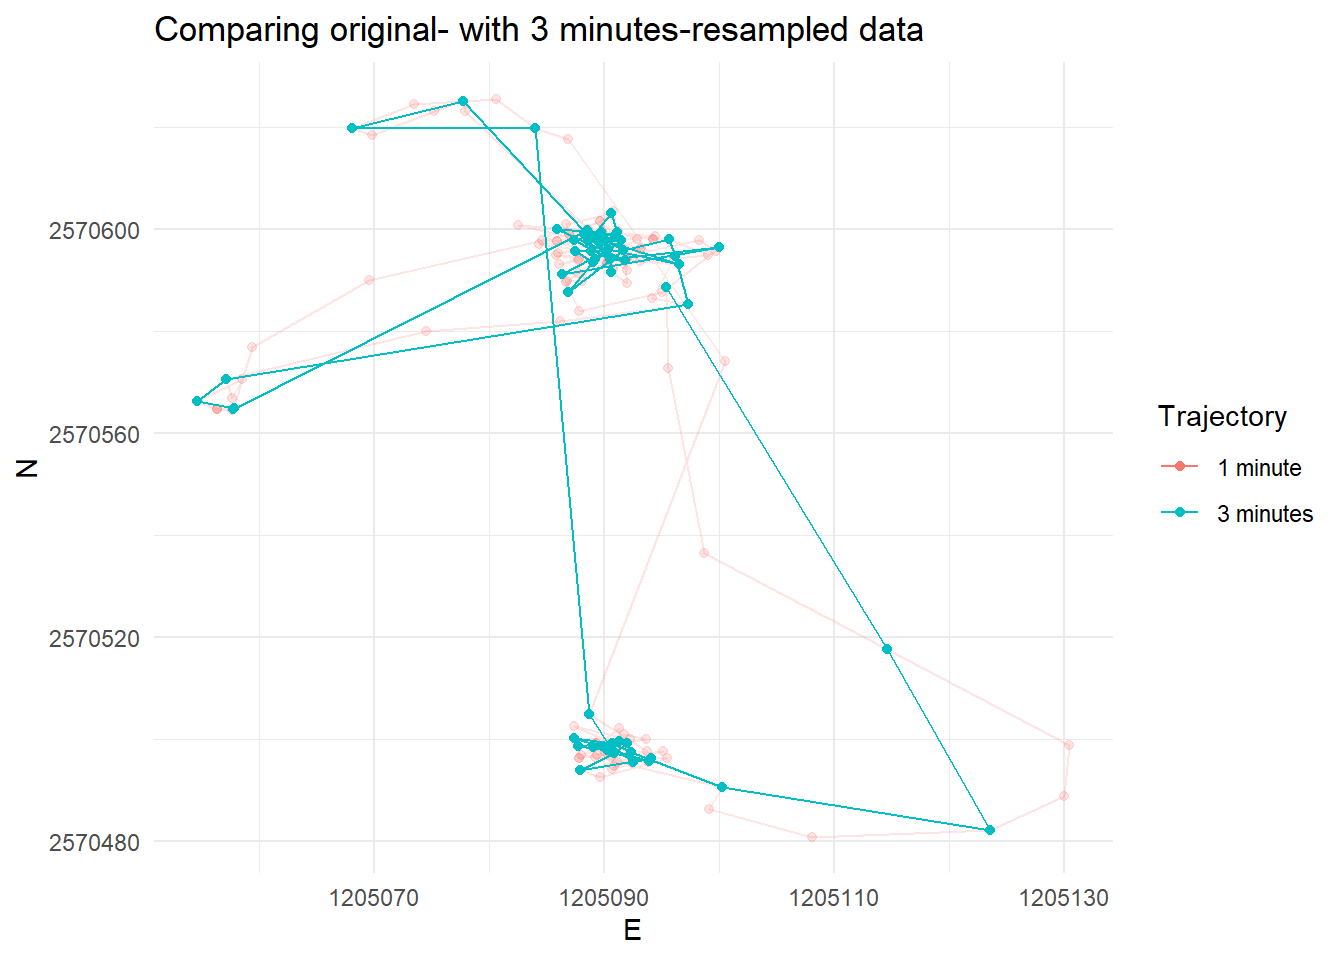
\includegraphics{_main_files/figure-latex/unnamed-chunk-58-1.pdf}
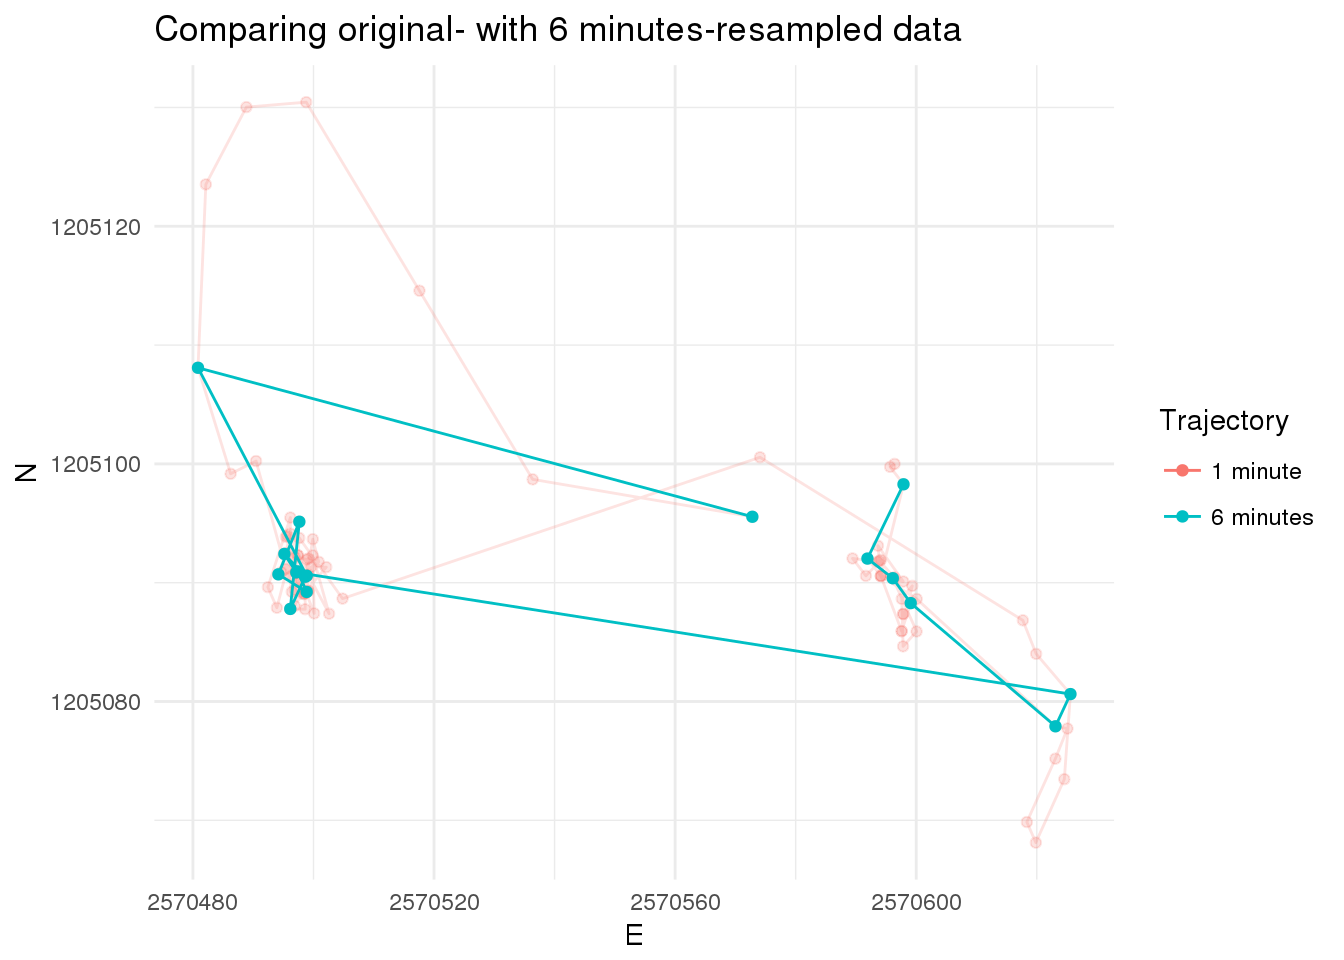
\includegraphics{_main_files/figure-latex/unnamed-chunk-58-2.pdf}
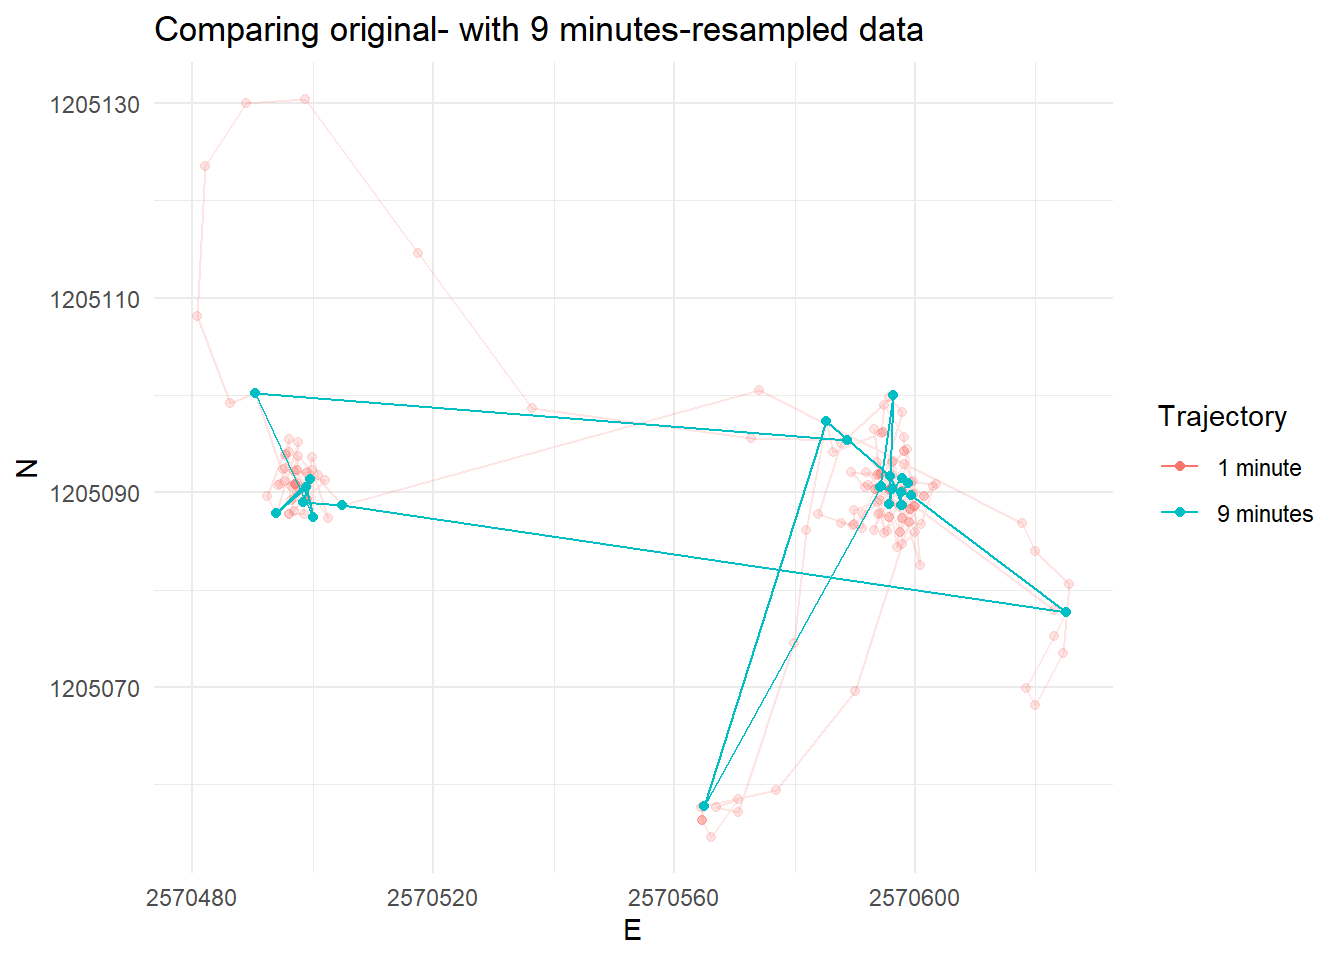
\includegraphics{_main_files/figure-latex/unnamed-chunk-58-3.pdf}
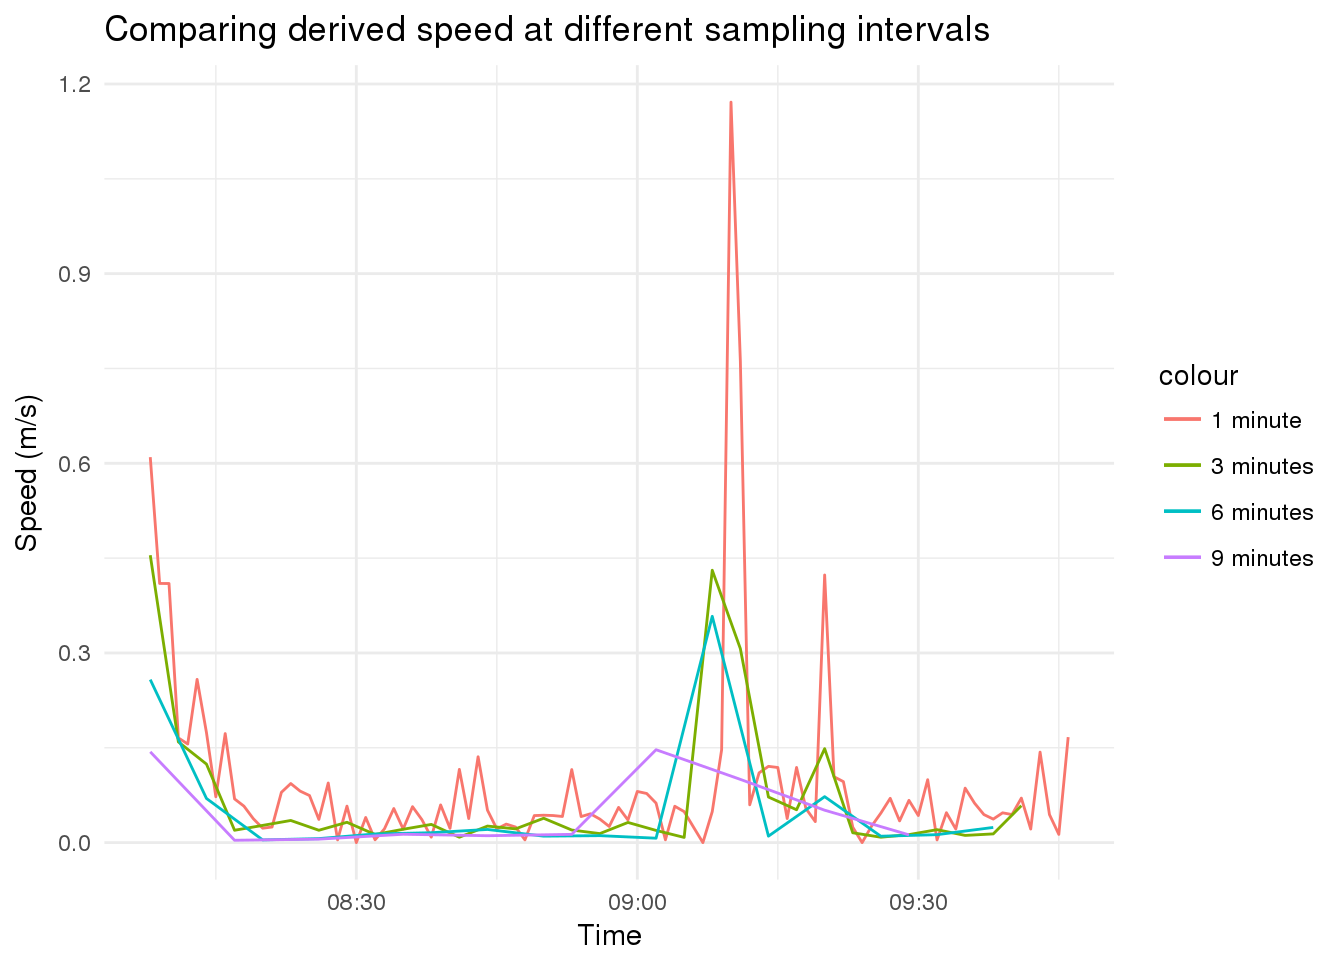
\includegraphics{_main_files/figure-latex/unnamed-chunk-58-4.pdf}

\subsection{Task 5 (Optional): Deriving movement parameters II: Rolling
window
functions}\label{task-5-optional-deriving-movement-parameters-ii-rolling-window-functions}

Measuring speed between subsequent samples is great, but especially for
short sampling intervals this can be misleading due to measurement
error. It might be desirable to \emph{smoothen} these errors using a
\href{https://docs.wavefront.com/images/5sec_moving_window.png}{moving
window function}. The \texttt{zoo} package offers a variate of moving
window functions (\texttt{roll*}). Use \texttt{roll\_mean()} to smooth
the calculated speed. Familiarise yourself with this function by working
on some dummy data, for example:

Visualize the output from your moving windows and compare different
window sizes (\texttt{k\ =}).

\section{Solutions (RCode)}\label{solutions-rcode}

\begin{Shaded}
\begin{Highlighting}[]
\NormalTok{## install.packages("zoo")}
\NormalTok{## }
\NormalTok{## devtools::install_git("https://github.engineering.zhaw.ch/PatternsTrendsEnvironmentalData/CMAtools.git")}
\NormalTok{wildschwein_BE <-}\StringTok{ }\KeywordTok{ungroup}\NormalTok{(wildschwein_BE)}
\NormalTok{## Demo Tidyverse ################}
\NormalTok{now <-}\StringTok{ }\KeywordTok{Sys.time}\NormalTok{()}

\NormalTok{later <-}\StringTok{ }\NormalTok{now +}\StringTok{ }\DecValTok{10000}

\KeywordTok{difftime}\NormalTok{(later,now)}
\NormalTok{time_difference <-}\StringTok{ }\KeywordTok{difftime}\NormalTok{(later,now,}\DataTypeTok{units =} \StringTok{"mins"}\NormalTok{)}

\NormalTok{time_difference}
\KeywordTok{str}\NormalTok{(time_difference)}
\NormalTok{time_difference <-}\StringTok{ }\KeywordTok{as.numeric}\NormalTok{(}\KeywordTok{difftime}\NormalTok{(later,now,}\DataTypeTok{units =} \StringTok{"mins"}\NormalTok{))}

\KeywordTok{str}\NormalTok{(time_difference)}

\NormalTok{numbers <-}\StringTok{ }\DecValTok{1}\NormalTok{:}\DecValTok{10}

\NormalTok{numbers}
\KeywordTok{lead}\NormalTok{(numbers)}

\KeywordTok{lead}\NormalTok{(numbers,}\DataTypeTok{n =} \DecValTok{2}\NormalTok{)}

\KeywordTok{lag}\NormalTok{(numbers)}

\KeywordTok{lag}\NormalTok{(numbers,}\DataTypeTok{n =} \DecValTok{5}\NormalTok{)}

\KeywordTok{lag}\NormalTok{(numbers,}\DataTypeTok{n =} \DecValTok{5}\NormalTok{, }\DataTypeTok{default =} \DecValTok{0}\NormalTok{)}
\KeywordTok{lead}\NormalTok{(numbers)-numbers}
\NormalTok{wildschwein_BE$timelag  <-}\StringTok{ }\KeywordTok{as.numeric}\NormalTok{(}\KeywordTok{difftime}\NormalTok{(}\KeywordTok{lead}\NormalTok{(wildschwein_BE$DatetimeUTC),wildschwein_BE$DatetimeUTC,}\DataTypeTok{units =} \StringTok{"secs"}\NormalTok{))}

\NormalTok{wildschwein_BE <-}\StringTok{ }\KeywordTok{mutate}\NormalTok{(wildschwein_BE,}\DataTypeTok{timelag =} \KeywordTok{as.numeric}\NormalTok{(}\KeywordTok{difftime}\NormalTok{(}\KeywordTok{lead}\NormalTok{(DatetimeUTC),DatetimeUTC,}\DataTypeTok{units =} \StringTok{"secs"}\NormalTok{)))}
\KeywordTok{summary}\NormalTok{(wildschwein_BE$timelag)}
\NormalTok{wildschwein_BE <-}\StringTok{ }\KeywordTok{group_by}\NormalTok{(wildschwein_BE,TierID)}
\NormalTok{wildschwein_BE <-}\StringTok{ }\KeywordTok{mutate}\NormalTok{(wildschwein_BE,}\DataTypeTok{timelag =} \KeywordTok{as.numeric}\NormalTok{(}\KeywordTok{difftime}\NormalTok{(}\KeywordTok{lead}\NormalTok{(DatetimeUTC),DatetimeUTC,}\DataTypeTok{units =} \StringTok{"secs"}\NormalTok{)))}

\KeywordTok{summary}\NormalTok{(wildschwein_BE$timelag)}
\NormalTok{## }
\NormalTok{## summarise(wildschwein_BE, mean = mean(timelag, na.rm = T))}
\NormalTok{## }
\KeywordTok{summarise}\NormalTok{(}\KeywordTok{group_by}\NormalTok{(}\KeywordTok{as.data.frame}\NormalTok{(wildschwein_BE),TierID), }\DataTypeTok{mean_timelag =} \KeywordTok{mean}\NormalTok{(timelag, }\DataTypeTok{na.rm =} \NormalTok{T))}

\NormalTok{wildschwein_BE %>%}\StringTok{                     }\CommentTok{# Take wildschwein_BE...}
\StringTok{  }\KeywordTok{as.data.frame}\NormalTok{() %>%}\StringTok{                  }\CommentTok{# ...convert it to a data.frame...}
\StringTok{  }\KeywordTok{group_by}\NormalTok{(TierID) %>%}\StringTok{                 }\CommentTok{# ...group it by TierID}
\StringTok{  }\KeywordTok{summarise}\NormalTok{(                           }\CommentTok{# Summarise the data..}
    \DataTypeTok{mean_timelag =} \KeywordTok{mean}\NormalTok{(timelag,}\DataTypeTok{na.rm =} \NormalTok{T) }\CommentTok{# ... by calculating the mean timelag}
  \NormalTok{)}
\NormalTok{## Task 1 ####################}

\KeywordTok{ggplot}\NormalTok{(wildschwein_BE, }\KeywordTok{aes}\NormalTok{(DatetimeUTC,TierID)) +}
\StringTok{  }\KeywordTok{geom_line}\NormalTok{()}

\KeywordTok{ggplot}\NormalTok{(wildschwein_BE, }\KeywordTok{aes}\NormalTok{(timelag)) +}
\StringTok{  }\KeywordTok{geom_histogram}\NormalTok{(}\DataTypeTok{binwidth =} \DecValTok{50}\NormalTok{)}

\KeywordTok{ggplot}\NormalTok{(wildschwein_BE, }\KeywordTok{aes}\NormalTok{(timelag)) +}
\StringTok{  }\KeywordTok{geom_histogram}\NormalTok{(}\DataTypeTok{binwidth =} \DecValTok{1}\NormalTok{) +}
\StringTok{  }\KeywordTok{lims}\NormalTok{(}\DataTypeTok{x =} \KeywordTok{c}\NormalTok{(}\DecValTok{0}\NormalTok{,}\DecValTok{100}\NormalTok{)) +}
\StringTok{  }\KeywordTok{scale_y_log10}\NormalTok{()}

\NormalTok{wildschwein_BE[}\DecValTok{1}\NormalTok{:}\DecValTok{50}\NormalTok{,] %>%}
\StringTok{  }\KeywordTok{ggplot}\NormalTok{(}\KeywordTok{aes}\NormalTok{(DatetimeUTC,timelag)) +}
\StringTok{  }\KeywordTok{geom_line}\NormalTok{() +}
\StringTok{  }\KeywordTok{geom_point}\NormalTok{()}


\NormalTok{## Input: cut vecotrs by intervals ####################}
\NormalTok{ages <-}\StringTok{ }\KeywordTok{c}\NormalTok{(}\DecValTok{20}\NormalTok{,}\DecValTok{25}\NormalTok{,}\DecValTok{18}\NormalTok{,}\DecValTok{13}\NormalTok{,}\DecValTok{53}\NormalTok{,}\DecValTok{50}\NormalTok{,}\DecValTok{23}\NormalTok{,}\DecValTok{43}\NormalTok{,}\DecValTok{68}\NormalTok{,}\DecValTok{40}\NormalTok{)}
\NormalTok{breaks <-}\StringTok{ }\KeywordTok{seq}\NormalTok{(}\DecValTok{0}\NormalTok{,}\DecValTok{50}\NormalTok{,}\DecValTok{10}\NormalTok{)}

\KeywordTok{cut}\NormalTok{(ages,}\DataTypeTok{breaks =} \NormalTok{breaks)}
\KeywordTok{cut}\NormalTok{(ages, }\DataTypeTok{breaks =} \KeywordTok{c}\NormalTok{(}\DecValTok{0}\NormalTok{,}\DecValTok{30}\NormalTok{,}\DecValTok{60}\NormalTok{,}\DecValTok{100}\NormalTok{), }\DataTypeTok{labels =} \KeywordTok{c}\NormalTok{(}\StringTok{"young"}\NormalTok{,}\StringTok{"middle aged"}\NormalTok{,}\StringTok{"old"}\NormalTok{))}
\NormalTok{## Task 2 ####################}

\NormalTok{breaks <-}\StringTok{ }\KeywordTok{c}\NormalTok{(}\DecValTok{0}\NormalTok{,}\DecValTok{40}\NormalTok{,}\DecValTok{80}\NormalTok{,}\DecValTok{300}\NormalTok{,}\DecValTok{600}\NormalTok{,}\DecValTok{1200}\NormalTok{,}\DecValTok{2500}\NormalTok{,}\DecValTok{3000}\NormalTok{,}\DecValTok{4000}\NormalTok{,}\DecValTok{7500}\NormalTok{,}\DecValTok{110000}\NormalTok{)}



\KeywordTok{ggplot}\NormalTok{(wildschwein_BE, }\KeywordTok{aes}\NormalTok{(timelag)) +}
\StringTok{  }\KeywordTok{geom_histogram}\NormalTok{(}\DataTypeTok{binwidth =} \DecValTok{10}\NormalTok{) +}
\StringTok{  }\KeywordTok{lims}\NormalTok{(}\DataTypeTok{x =} \KeywordTok{c}\NormalTok{(}\DecValTok{0}\NormalTok{,}\DecValTok{600}\NormalTok{)) +}
\StringTok{  }\KeywordTok{scale_y_log10}\NormalTok{() +}
\StringTok{  }\KeywordTok{geom_vline}\NormalTok{(}\DataTypeTok{xintercept =} \NormalTok{breaks, }\DataTypeTok{col =} \StringTok{"red"}\NormalTok{)}

\KeywordTok{ggplot}\NormalTok{(wildschwein_BE, }\KeywordTok{aes}\NormalTok{(timelag)) +}
\StringTok{  }\KeywordTok{geom_histogram}\NormalTok{(}\DataTypeTok{binwidth =} \DecValTok{10}\NormalTok{) +}
\StringTok{  }\KeywordTok{lims}\NormalTok{(}\DataTypeTok{x =} \KeywordTok{c}\NormalTok{(}\DecValTok{600}\NormalTok{,}\DecValTok{1200}\NormalTok{)) +}
\StringTok{  }\KeywordTok{scale_y_log10}\NormalTok{() +}
\StringTok{  }\KeywordTok{geom_vline}\NormalTok{(}\DataTypeTok{xintercept =} \NormalTok{breaks, }\DataTypeTok{col =} \StringTok{"red"}\NormalTok{)}


\KeywordTok{ggplot}\NormalTok{(wildschwein_BE, }\KeywordTok{aes}\NormalTok{(timelag)) +}
\StringTok{  }\KeywordTok{geom_histogram}\NormalTok{(}\DataTypeTok{binwidth =} \DecValTok{10}\NormalTok{) +}
\StringTok{  }\KeywordTok{lims}\NormalTok{(}\DataTypeTok{x =} \KeywordTok{c}\NormalTok{(}\DecValTok{1200}\NormalTok{,}\DecValTok{10000}\NormalTok{)) +}
\StringTok{  }\KeywordTok{scale_y_log10}\NormalTok{() +}
\StringTok{  }\KeywordTok{geom_vline}\NormalTok{(}\DataTypeTok{xintercept =} \NormalTok{breaks, }\DataTypeTok{col =} \StringTok{"red"}\NormalTok{)}

\NormalTok{labels_nice <-}\StringTok{ }\NormalTok{function(breaks)\{}
  \KeywordTok{return}\NormalTok{(}\KeywordTok{paste}\NormalTok{(}\KeywordTok{lag}\NormalTok{(breaks,}\DataTypeTok{default =} \OtherTok{NULL}\NormalTok{),}\KeywordTok{lead}\NormalTok{(breaks,}\DataTypeTok{default =} \OtherTok{NULL}\NormalTok{),}\DataTypeTok{sep=}\StringTok{"-"}\NormalTok{))}
\NormalTok{\}}

\CommentTok{# todo: noch in CMA Tools integrieren}


\NormalTok{wildschwein_BE <-}\StringTok{ }\NormalTok{wildschwein_BE %>%}
\StringTok{  }\KeywordTok{group_by}\NormalTok{(TierID) %>%}
\StringTok{  }\KeywordTok{mutate}\NormalTok{(}
    \DataTypeTok{samplingInt =} \KeywordTok{cut}\NormalTok{(timelag,}\DataTypeTok{breaks =} \NormalTok{breaks,}\DataTypeTok{labels =} \KeywordTok{labels_nice}\NormalTok{(breaks))}
  \NormalTok{) }

\NormalTok{wildschwein_BE %>%}
\StringTok{  }\KeywordTok{as.data.frame}\NormalTok{() %>%}
\StringTok{  }\KeywordTok{group_by}\NormalTok{(samplingInt) %>%}
\StringTok{  }\KeywordTok{summarise}\NormalTok{(}
    \DataTypeTok{n =} \KeywordTok{n}\NormalTok{()}
  \NormalTok{) %>%}
\StringTok{  }\KeywordTok{ggplot}\NormalTok{(}\KeywordTok{aes}\NormalTok{(samplingInt,n)) +}
\StringTok{  }\KeywordTok{geom_bar}\NormalTok{(}\DataTypeTok{stat =} \StringTok{"identity"}\NormalTok{) +}
\StringTok{  }\KeywordTok{theme}\NormalTok{(}\DataTypeTok{axis.text.x =} \KeywordTok{element_text}\NormalTok{(}\DataTypeTok{angle =} \DecValTok{45}\NormalTok{, }\DataTypeTok{hjust =} \DecValTok{1}\NormalTok{)) +}
\StringTok{  }\KeywordTok{scale_y_log10}\NormalTok{()}



\NormalTok{wildschwein_BE}

\CommentTok{# Store coordinates in a new variable}
\NormalTok{coordinates <-}\StringTok{ }\KeywordTok{st_coordinates}\NormalTok{(wildschwein_BE)}

\KeywordTok{head}\NormalTok{(coordinates)}
\KeywordTok{colnames}\NormalTok{(coordinates) <-}\StringTok{ }\KeywordTok{c}\NormalTok{(}\StringTok{"E"}\NormalTok{,}\StringTok{"N"}\NormalTok{)}

\NormalTok{wildschwein_BE <-}\StringTok{ }\KeywordTok{cbind}\NormalTok{(wildschwein_BE,coordinates)}
\NormalTok{## Task 3 ####################}

\KeywordTok{library}\NormalTok{(CMAtools)}

\NormalTok{wildschwein_BE <-}\StringTok{ }\NormalTok{wildschwein_BE %>%}
\StringTok{  }\KeywordTok{group_by}\NormalTok{(TierID,samplingInt) %>%}
\StringTok{  }\KeywordTok{mutate}\NormalTok{(}
    \DataTypeTok{steplength =} \KeywordTok{euclid}\NormalTok{(}\KeywordTok{lead}\NormalTok{(E, }\DecValTok{1}\NormalTok{),}\KeywordTok{lead}\NormalTok{(N, }\DecValTok{1}\NormalTok{),E,N),}
    \DataTypeTok{speed =} \NormalTok{steplength/timelag}
  \NormalTok{)}



\NormalTok{sample <-}\StringTok{ }\KeywordTok{data.frame}\NormalTok{(}\DataTypeTok{position =} \KeywordTok{paste0}\NormalTok{(}\StringTok{"pos"}\NormalTok{,}\DecValTok{1}\NormalTok{:}\DecValTok{6}\NormalTok{),}\DataTypeTok{samplingInt=}\KeywordTok{c}\NormalTok{(}\KeywordTok{rep}\NormalTok{(}\DecValTok{60}\NormalTok{,}\DecValTok{3}\NormalTok{),}\KeywordTok{rep}\NormalTok{(}\DecValTok{120}\NormalTok{,}\DecValTok{3}\NormalTok{)))}
\NormalTok{sample}
\NormalTok{sample <-}\StringTok{ }\NormalTok{sample %>%}
\StringTok{  }\KeywordTok{mutate}\NormalTok{(}
    \DataTypeTok{samplingInt_control =} \NormalTok{samplingInt ==}\StringTok{ }\KeywordTok{lead}\NormalTok{(samplingInt,}\DecValTok{1}\NormalTok{),}
    \DataTypeTok{samplingInt_group =} \KeywordTok{number_groups}\NormalTok{(samplingInt_control,}\DataTypeTok{include_first_false =} \NormalTok{T)}
  \NormalTok{)}

\NormalTok{sample}
\NormalTok{wildschwein_BE <-}\StringTok{ }\NormalTok{wildschwein_BE %>%}
\StringTok{  }\KeywordTok{group_by}\NormalTok{(TierID) %>%}
\StringTok{  }\KeywordTok{mutate}\NormalTok{(}
    \DataTypeTok{samplingInt_T =} \NormalTok{samplingInt ==}\StringTok{ }\KeywordTok{lead}\NormalTok{(samplingInt),}
    \DataTypeTok{group =} \KeywordTok{number_groups}\NormalTok{(samplingInt_T,}\DataTypeTok{include_first_false =} \NormalTok{T)}
  \NormalTok{) %>%}
\StringTok{  }\NormalTok{dplyr::}\KeywordTok{select}\NormalTok{(-samplingInt_T)}

\NormalTok{wildschwein_BE_short <-}\StringTok{ }\NormalTok{wildschwein_BE %>%}
\StringTok{  }\KeywordTok{filter}\NormalTok{(samplingInt ==}\StringTok{ "40-80"}\NormalTok{)}

\NormalTok{wildschwein_BE_short <-}\StringTok{ }\NormalTok{wildschwein_BE_short %>%}
\StringTok{  }\KeywordTok{filter}\NormalTok{(group ==}\StringTok{ }\DecValTok{9}\NormalTok{) %>%}
\StringTok{  }\KeywordTok{slice}\NormalTok{(}\DecValTok{1}\NormalTok{:}\DecValTok{100}\NormalTok{)}


\NormalTok{wildschwein_BE_3 <-}\StringTok{ }\NormalTok{wildschwein_BE_short %>%}
\StringTok{  }\KeywordTok{slice}\NormalTok{(}\KeywordTok{seq}\NormalTok{(}\DecValTok{1}\NormalTok{,}\KeywordTok{nrow}\NormalTok{(.),}\DecValTok{3}\NormalTok{))}

\NormalTok{wildschwein_BE_6 <-}\StringTok{ }\NormalTok{wildschwein_BE_short %>%}
\StringTok{  }\KeywordTok{slice}\NormalTok{(}\KeywordTok{seq}\NormalTok{(}\DecValTok{1}\NormalTok{,}\KeywordTok{nrow}\NormalTok{(.),}\DecValTok{6}\NormalTok{))}


\NormalTok{wildschwein_BE_9 <-}\StringTok{ }\NormalTok{wildschwein_BE_short %>%}
\StringTok{  }\KeywordTok{slice}\NormalTok{(}\KeywordTok{seq}\NormalTok{(}\DecValTok{1}\NormalTok{,}\KeywordTok{nrow}\NormalTok{(.),}\DecValTok{9}\NormalTok{))}

\NormalTok{wildschwein_BE_3 <-}\StringTok{ }\NormalTok{wildschwein_BE_3 %>%}
\StringTok{  }\KeywordTok{mutate}\NormalTok{(}
    \DataTypeTok{timelag =} \KeywordTok{as.numeric}\NormalTok{(}\KeywordTok{difftime}\NormalTok{(}\KeywordTok{lead}\NormalTok{(DatetimeUTC),DatetimeUTC,}\DataTypeTok{units =} \StringTok{"secs"}\NormalTok{)),}
    \DataTypeTok{steplength =} \KeywordTok{euclid}\NormalTok{(}\KeywordTok{lead}\NormalTok{(E, }\DecValTok{1}\NormalTok{),}\KeywordTok{lead}\NormalTok{(N, }\DecValTok{1}\NormalTok{),E,N),}
    \DataTypeTok{speed =} \NormalTok{steplength/timelag}
  \NormalTok{)}

\NormalTok{wildschwein_BE_6 <-}\StringTok{ }\NormalTok{wildschwein_BE_6 %>%}
\StringTok{  }\KeywordTok{mutate}\NormalTok{(}
    \DataTypeTok{timelag =} \KeywordTok{as.numeric}\NormalTok{(}\KeywordTok{difftime}\NormalTok{(}\KeywordTok{lead}\NormalTok{(DatetimeUTC),DatetimeUTC,}\DataTypeTok{units =} \StringTok{"secs"}\NormalTok{)),}
    \DataTypeTok{steplength =} \KeywordTok{euclid}\NormalTok{(}\KeywordTok{lead}\NormalTok{(E, }\DecValTok{1}\NormalTok{),}\KeywordTok{lead}\NormalTok{(N, }\DecValTok{1}\NormalTok{),E,N),}
    \DataTypeTok{speed =} \NormalTok{steplength/timelag}
  \NormalTok{)}


\NormalTok{wildschwein_BE_9 <-}\StringTok{ }\NormalTok{wildschwein_BE_9 %>%}
\StringTok{  }\KeywordTok{mutate}\NormalTok{(}
    \DataTypeTok{timelag =} \KeywordTok{as.numeric}\NormalTok{(}\KeywordTok{difftime}\NormalTok{(}\KeywordTok{lead}\NormalTok{(DatetimeUTC),DatetimeUTC,}\DataTypeTok{units =} \StringTok{"secs"}\NormalTok{)),}
    \DataTypeTok{steplength =} \KeywordTok{euclid}\NormalTok{(}\KeywordTok{lead}\NormalTok{(E, }\DecValTok{1}\NormalTok{),}\KeywordTok{lead}\NormalTok{(N, }\DecValTok{1}\NormalTok{),E,N),}
    \DataTypeTok{speed =} \NormalTok{steplength/timelag}
  \NormalTok{)}


\KeywordTok{ggplot}\NormalTok{() +}
\StringTok{  }\KeywordTok{geom_point}\NormalTok{(}\DataTypeTok{data =} \NormalTok{wildschwein_BE_9, }\KeywordTok{aes}\NormalTok{(E,N), }\DataTypeTok{colour =} \StringTok{"red"}\NormalTok{) +}
\StringTok{  }\KeywordTok{geom_path}\NormalTok{(}\DataTypeTok{data =} \NormalTok{wildschwein_BE_9, }\KeywordTok{aes}\NormalTok{(E,N), }\DataTypeTok{colour =} \StringTok{"red"}\NormalTok{) +}
\StringTok{  }\KeywordTok{geom_point}\NormalTok{(}\DataTypeTok{data =} \NormalTok{wildschwein_BE_6, }\KeywordTok{aes}\NormalTok{(E,N), }\DataTypeTok{colour =} \StringTok{"blue"}\NormalTok{) +}
\StringTok{  }\KeywordTok{geom_path}\NormalTok{(}\DataTypeTok{data =} \NormalTok{wildschwein_BE_6, }\KeywordTok{aes}\NormalTok{(E,N), }\DataTypeTok{colour =} \StringTok{"blue"}\NormalTok{) +}
\StringTok{  }\KeywordTok{geom_point}\NormalTok{(}\DataTypeTok{data =} \NormalTok{wildschwein_BE_3, }\KeywordTok{aes}\NormalTok{(E,N), }\DataTypeTok{colour =} \StringTok{"green"}\NormalTok{) +}
\StringTok{  }\KeywordTok{geom_path}\NormalTok{(}\DataTypeTok{data =} \NormalTok{wildschwein_BE_3, }\KeywordTok{aes}\NormalTok{(E,N), }\DataTypeTok{colour =} \StringTok{"green"}\NormalTok{) +}
\StringTok{  }\KeywordTok{geom_point}\NormalTok{(}\DataTypeTok{data =} \NormalTok{wildschwein_BE_short, }\KeywordTok{aes}\NormalTok{(E,N), }\DataTypeTok{colour =} \StringTok{"black"}\NormalTok{) +}
\StringTok{  }\KeywordTok{geom_path}\NormalTok{(}\DataTypeTok{data =} \NormalTok{wildschwein_BE_short, }\KeywordTok{aes}\NormalTok{(E,N), }\DataTypeTok{colour =} \StringTok{"black"}\NormalTok{)}


\KeywordTok{ggplot}\NormalTok{() +}
\StringTok{  }\KeywordTok{geom_point}\NormalTok{(}\DataTypeTok{data =} \NormalTok{wildschwein_BE_9, }\KeywordTok{aes}\NormalTok{(DatetimeUTC,speed), }\DataTypeTok{colour =} \StringTok{"red"}\NormalTok{) +}
\StringTok{  }\KeywordTok{geom_path}\NormalTok{(}\DataTypeTok{data =} \NormalTok{wildschwein_BE_9, }\KeywordTok{aes}\NormalTok{(DatetimeUTC,speed), }\DataTypeTok{colour =} \StringTok{"red"}\NormalTok{) +}
\StringTok{  }\KeywordTok{geom_point}\NormalTok{(}\DataTypeTok{data =} \NormalTok{wildschwein_BE_6, }\KeywordTok{aes}\NormalTok{(DatetimeUTC,speed), }\DataTypeTok{colour =} \StringTok{"blue"}\NormalTok{) +}
\StringTok{  }\KeywordTok{geom_path}\NormalTok{(}\DataTypeTok{data =} \NormalTok{wildschwein_BE_6, }\KeywordTok{aes}\NormalTok{(DatetimeUTC,speed), }\DataTypeTok{colour =} \StringTok{"blue"}\NormalTok{) +}
\StringTok{  }\KeywordTok{geom_point}\NormalTok{(}\DataTypeTok{data =} \NormalTok{wildschwein_BE_3, }\KeywordTok{aes}\NormalTok{(DatetimeUTC,speed), }\DataTypeTok{colour =} \StringTok{"green"}\NormalTok{) +}
\StringTok{  }\KeywordTok{geom_path}\NormalTok{(}\DataTypeTok{data =} \NormalTok{wildschwein_BE_3, }\KeywordTok{aes}\NormalTok{(DatetimeUTC,speed), }\DataTypeTok{colour =} \StringTok{"green"}\NormalTok{) +}
\StringTok{  }\KeywordTok{geom_point}\NormalTok{(}\DataTypeTok{data =} \NormalTok{wildschwein_BE_short, }\KeywordTok{aes}\NormalTok{(DatetimeUTC,speed), }\DataTypeTok{colour =} \StringTok{"black"}\NormalTok{) +}
\StringTok{  }\KeywordTok{geom_path}\NormalTok{(}\DataTypeTok{data =} \NormalTok{wildschwein_BE_short, }\KeywordTok{aes}\NormalTok{(DatetimeUTC,speed), }\DataTypeTok{colour =} \StringTok{"black"}\NormalTok{) +}
\StringTok{  }\KeywordTok{labs}\NormalTok{(}\DataTypeTok{x =} \StringTok{"Time"}\NormalTok{,}\DataTypeTok{y =} \StringTok{"Speed (m/s)"}\NormalTok{)}

\NormalTok{## Task 4 ####################}

\KeywordTok{library}\NormalTok{(zoo)}

\NormalTok{example <-}\StringTok{ }\KeywordTok{rnorm}\NormalTok{(}\DecValTok{10}\NormalTok{)}
\KeywordTok{rollmean}\NormalTok{(example,}\DataTypeTok{k =} \DecValTok{3}\NormalTok{,}\DataTypeTok{fill =} \OtherTok{NA}\NormalTok{,}\DataTypeTok{align =} \StringTok{"left"}\NormalTok{)}
\KeywordTok{rollmean}\NormalTok{(example,}\DataTypeTok{k =} \DecValTok{4}\NormalTok{,}\DataTypeTok{fill =} \OtherTok{NA}\NormalTok{,}\DataTypeTok{align =} \StringTok{"left"}\NormalTok{)}



\NormalTok{wildschwein_BE <-}\StringTok{ }\NormalTok{wildschwein_BE %>%}
\StringTok{  }\KeywordTok{group_by}\NormalTok{(TierID) %>%}
\StringTok{  }\KeywordTok{mutate}\NormalTok{(}
    \DataTypeTok{speed2 =} \KeywordTok{rollmean}\NormalTok{(speed,}\DecValTok{3}\NormalTok{,}\OtherTok{NA}\NormalTok{,}\DataTypeTok{align =} \StringTok{"left"}\NormalTok{),}
    \DataTypeTok{speed3 =} \KeywordTok{rollmean}\NormalTok{(speed,}\DecValTok{5}\NormalTok{,}\OtherTok{NA}\NormalTok{,}\DataTypeTok{align =} \StringTok{"left"}\NormalTok{),}
    \DataTypeTok{speed4 =} \KeywordTok{rollmean}\NormalTok{(speed,}\DecValTok{10}\NormalTok{,}\OtherTok{NA}\NormalTok{,}\DataTypeTok{align =} \StringTok{"left"}\NormalTok{)}
  \NormalTok{)}

\NormalTok{wildschwein_BE[}\DecValTok{1}\NormalTok{:}\DecValTok{30}\NormalTok{,] %>%}
\StringTok{  }\KeywordTok{gather}\NormalTok{(key,val,}\KeywordTok{c}\NormalTok{(speed,speed2,speed3,speed4)) %>%}
\StringTok{  }\KeywordTok{ggplot}\NormalTok{(}\KeywordTok{aes}\NormalTok{(DatetimeUTC,val,}\DataTypeTok{colour =} \NormalTok{key,}\DataTypeTok{group =} \NormalTok{key)) +}
\StringTok{  }\KeywordTok{geom_point}\NormalTok{() +}
\StringTok{  }\KeywordTok{geom_line}\NormalTok{() }
\NormalTok{## NA}
\end{Highlighting}
\end{Shaded}

\hypertarget{refs}{}
\hypertarget{ref-laube2011}{}
Laube, Patrick, and Ross S. Purves. 2011. ``How Fast Is a Cow? Cross -
Scale Analysis of Movement Data.'' \emph{Transactions in GIS} 15 (3):
401--18.
doi:\href{https://doi.org/10.1111/j.1467-9671.2011.01256.x}{10.1111/j.1467-9671.2011.01256.x}.

\hypertarget{ref-wickham2017}{}
Wickham, Hadley, and Garrett Grolemund. 2017. \emph{R for Data Science:
Import, Tidy, Transform, Visualize, and Model Data}. 1st ed. O'Reilly
Media, Inc.


\end{document}
